\chapter*{ECRICOME 2016 : le corrigé}
  
%

\section*{EXERCICE 1}

\subsection*{Partie A}

\noindent Pour tout couple de réels $(x,y)$, on définit la matrice 
$M(x,y)$ par~:
\[ 
M(x,y) = 
\begin{smatrix} 
3x & -2x+2y & 2x - y \\ 
-x-y & 4x-3y & -2x+y \\
-2y & 4x-4y & -x+y 
\end{smatrix}
\]
On appelle $E$ l'ensemble des matrices $M(x,y)$ où $x$ et $y$ décrivent 
$\R$~:
\[ 
E = \{ M(x,y), \ (x,y) \in \R^2 \} 
\]
On note $A = M(1,0)$ et $B=M(0,1)$.
\begin{noliste}{1.}
 \setlength{\itemsep}{2mm}
 \item Montrer que $E$ est un sous-espace vectoriel de 
 $\M{3}$.\\ 
 En déterminer une base et donner sa 
 dimension.
 
 \begin{proof}~
  \begin{noliste}{$\sbullet$}
    \item Par définition de $E$, on a :
    \[
     \begin{array}{rcl}
      E & = & \{ M(x,y), \ (x,y)\in \R^2\}
      \\[.4cm]
      & = & \{
      \begin{smatrix}
       3x & -2x+2y & 2x-y \\
       -x-y & 4x-3y & -2x+y \\
       -2y & 4x-4y & -x+y 
      \end{smatrix}
      \ | \ (x,y)\in\R^2
      \}
      \\[.8cm]
      & = & \{ x\cdot
      \begin{smatrix}
       3 & -2 & 2\\
       -1 & 4 & -2\\
       0 & 4 & -1
      \end{smatrix}
      + y\cdot
      \begin{smatrix}
       0 & 2 & -1\\
       -1 & -3 & 1\\
       -2 & -4 & 1
      \end{smatrix}
      \ | \ (x,y)\in\R^2 \}
      \\[.8cm]
      & = & \{ x\cdot M(1,0)
      + y\cdot M(0,1)
      \ | \ (x,y)\in\R^2 \}
      \\[.4cm]
      & = & \{ x\cdot A
      + y\cdot B
      \ | \ (x,y)\in\R^2 \}
      \\[.4cm]
      & = & \Vect{A, B}
     \end{array}
    \]
    De plus, $(A,B) \in (\M{3})^2$.
    \conc{Donc $E$ est un sous-espace vectoriel de $\M{3}$.}
    
    \item La famille $(A,B)$ :
    \begin{noliste}{$\stimes$}
      \item engendre $E$ (d'après le point précédent),
      \item est libre dans $\M{3}$, car elle est constituée de $2$ 
      matrices non proportionnelles.
    \end{noliste}
    \conc{D'où $(A,B)$ est une base de $E$.}
    
    \item Déterminons la dimension de $E$.
    \conc{$\dim(E)=\Card((A,B))=2$}
  \end{noliste}
  
  \newpage
  
  \begin{remark}
   Deux méthodes sont à disposition pour montrer qu'un ensemble $F$ est 
   un sous-espace vectoriel d'un espace vectoriel $E$.
   \begin{noliste}{$\sbullet$}
    \item Utiliser la définition d'un sous-espace vectoriel de $E$ :
    \begin{noliste}{\scriptsize 1.}
      \item Montrer que $F \subset E$.
      \item Montrer que $0_E \in F$.
      \item Montrer que : 
      \[
      \forall (\lambda_1, \lambda_2) \in \R^2, \ 
      \forall (u_1,u_2)\in F^2, \quad 
      \lambda_1 \cdot u_1 + \lambda_2 \cdot u_2 \in F
      \]
    \end{noliste}
    \item Montrer que $F$ s'écrit comme un sous-espace vectoriel 
    engendré par une famille d'éléments de $E$ (c'est la méthode 
    employée dans cette question).
   \end{noliste}
   On privilégiera la seconde méthode dès que possible. En
   particulier, si l'énoncé demande une base de $F$, il est certain
   qu'il faut exprimer $F$ comme un sous-espace vectoriel engendré par
   une famille de $E$. Par défaut (et par défaut seulement), on
   utilisera la définition d'un sous-espace vectoriel.
  \end{remark}~\\[-1.4cm]
 \end{proof}


 \item Montrer que $1$, $2$ et $3$ sont valeurs propres de $A$ et 
 déterminer les espaces propres associés.\\ 
 $A$ est-elle diagonalisable~?
 
 \begin{proof}~
  \begin{noliste}{$\sbullet$}
  \item Déterminons $E_1(A) = \{X \in \M{3,1} \ | \ (A-1 \cdot I_3) \
    X = 0_{\M{3,1}} \}$.\\
    Soit $X=
   \begin{smatrix}
    x\\
    y\\
    z
   \end{smatrix}\in \M{3,1}$.
   \[
    \begin{array}{rcl}
      X\in E_1(A) & \Longleftrightarrow & (A-1 \cdot I_3) \ X = 0_{\M{3,1}}
      \\[.2cm]
      & \Longleftrightarrow & 
     \begin{smatrix}
      2 & -2 & 2\\
      -1 & 3 & -2\\
      0 & 4 & -2
     \end{smatrix}
     \begin{smatrix}
      x\\
      y\\
      z
     \end{smatrix}
     =
     \begin{smatrix}
      0\\
      0\\
      0
     \end{smatrix}
     \\[.8cm]
     & \Longleftrightarrow &
     \left\{
     \begin{array}{rrrrrcl}
      2x & - & 2y & + & 2z & = & 0\\
      -x & + & 3y & - & 2z & = & 0\\
      & & 4y & - & 2z & = & 0
     \end{array}
     \right.
     \\[.8cm]
     &
     \begin{arrayEq}
      L_1 \leftarrow \frac{1}{2} \, L_1\\[.2cm]
      L_3 \leftarrow \frac{1}{2} \, L_3
     \end{arrayEq}
     &
     \left\{
     \begin{array}{rrrrrcl}
      x & - & y & + & z & = & 0\\
      -x & + & 3y & - & 2z & = & 0\\
      & & 2y & - & z & = & 0
     \end{array}
     \right.
     \\[.8cm]
     &
     \begin{arrayEq}
      L_2 \leftarrow L_2 + L_1
     \end{arrayEq}
     &
     \left\{
     \begin{array}{rrrrrcl}
      x & - & y & + & z & = & 0\\
      & & 2y & - & z & = & 0\\
      & & 2y & - & z & = & 0
     \end{array}
     \right.
     \\[.8cm]
     & \Longleftrightarrow &
     \left\{
     \begin{array}{rrrrrcl}
      x & - & y & + & z & = & 0\\
      & & 2y & - & z & = & 0
     \end{array}
     \right.
     \\[.6cm]
     & \Longleftrightarrow & 
     \left\{
     \begin{array}{rrrcr}
      x & - & y & = & -z\\
      & & 2y & = & z
     \end{array}
     \right.
     \\[.6cm]
     &
     \begin{arrayEq}
      L_1 \leftarrow 2 \, L_1 + L_2
     \end{arrayEq}
     &
     \left\{
     \begin{array}{rrrcr}
      2x & & & = & -z\\
      & & 2y & = & z
     \end{array}
     \right.
     \ \Longleftrightarrow \
     \left\{
     \begin{array}{rcr}
       x & = & -\frac{1}{2} \, z\\[.2cm]
       y & = & \frac{1}{2} \, z
     \end{array}
     \right.
    \end{array}
   \]
   

   \newpage


   \noindent
   Finalement, on obtient l'expression de $E_1(A)$ suivante :
   \[
    \begin{array}{rcl}
     E_1(A) & = & \{
     \begin{smatrix}
      x\\
      y\\
      z
     \end{smatrix}
     \in \M{3,1} \ | \ x=-\dfrac{1}{2} \, z \mbox{ et } y=\dfrac{1}{2} 
     \, z \}
     \\[.6cm]
     & = & \{
     \begin{smatrix}
      -\frac{1}{2} \, z\\[.2cm]
      \frac{1}{2} \, z\\[.2cm]
      z
     \end{smatrix}
     \ | \ z\in\R \}
     \ = \ \{ z \cdot
     \begin{smatrix}
      -\frac{1}{2}\\[.2cm]
      \frac{1}{2}\\[.2cm]
      1
     \end{smatrix}
     \ | \ z\in\R \}
     %\\[.8cm]
     \ = \ \Vect{
     \begin{smatrix}
      -\frac{1}{2}\\[.2cm]
      \frac{1}{2}\\[.2cm]
      1
     \end{smatrix}
     }
%      \ = \ \Vect{
%      \begin{smatrix}
%       1\\[.2cm]
%       -1\\[.2cm]
%       -2
%      \end{smatrix}
%      }
    \end{array}
   \]   
   Comme $E_1(A) \neq \{0_{\M{3,1}}\}$, $1$ est bien valeur propre de
   $A$, d'espace propre associé $E_1(A)$.%
   \conc{$E_1(A) \ = \ \Vect{
       \begin{smatrix}
         -\frac{1}{2} \\[.2cm]
         \frac{1}{2} \\[.2cm]
         1
       \end{smatrix}
     } \ = \ \Vect{
       \begin{smatrix}
         1\\[.2cm]
         -1\\[.2cm]
         -2
       \end{smatrix}
     }$}
   
 \item Déterminons $E_2(A) = \{X \in \M{3,1} \ | \ (A - 2 \cdot I_3) \
    X = 0_{\M{3,1}} \}$.\\
   Soit $X=
   \begin{smatrix}
    x\\
    y\\
    z
   \end{smatrix}\in \M{3,1}$.
   \[
    \begin{array}{rcl}
      X\in E_2(A) & \Longleftrightarrow & (A-2 \cdot I_3) \ X = 0_{\M{3,1}}
      \\[.2cm]
      & \Longleftrightarrow & 
     \begin{smatrix}
      1 & -2 & 2\\
      -1 & 2 & -2\\
      0 & 4 & -3
     \end{smatrix}
     \begin{smatrix}
      x\\
      y\\
      z
     \end{smatrix}
     =
     \begin{smatrix}
      0\\
      0\\
      0
     \end{smatrix}
     \\[.8cm]
     & \Longleftrightarrow &
     \left\{
     \begin{array}{rrrrrcl}
      x & - & 2y & + & 2z & = & 0\\
      -x & + & 2y & - & 2z & = & 0\\
      & & 4y & - & 3z & = & 0
     \end{array}
     \right.
     \\[.8cm]
     &
     \begin{arrayEq}
      L_2 \leftarrow L_2 + L_1
     \end{arrayEq}
     &
     \left\{
     \begin{array}{rrrrrcl}
      x & - & 2y & + & 2z & = & 0\\
      & & 4y & - & 3z & = & 0
     \end{array}
     \right.
     \\[.6cm]
     & \Longleftrightarrow & 
     \left\{
     \begin{array}{rrrcr}
      x & - & 2y & = & -2z\\
      & & 4y & = & 3z
     \end{array}
     \right.
     \\[.6cm]
     &
     \begin{arrayEq}
      L_1 \leftarrow 2 \, L_1 + L_2
     \end{arrayEq}
     &
     \left\{
     \begin{array}{rrrcr}
      2x & & & = & -z\\
      & & 4y & = & 3z
     \end{array}
     \right.
     \ \Longleftrightarrow \
     \left\{
     \begin{array}{rcr}
      x & = & -\frac{1}{2} \, z\\[.2cm]
      y & = & \frac{3}{4} \, z
     \end{array}
     \right.
    \end{array}
   \]   
   Finalement, on obtient l'expression de $E_2(A)$ suivante :
   \[
    \begin{array}{rcl}
     E_2(A) & = & \{
     \begin{smatrix}
      x\\
      y\\
      z
     \end{smatrix}
     \in \M{3,1} \ | \ x=-\dfrac{1}{2} \, z \mbox{ et } y=\dfrac{3}{4} 
     \, z \}
     \\[.6cm]
     & = & \{
     \begin{smatrix}
      -\frac{1}{2} \, z\\[.2cm]
      \frac{3}{4} \, z\\[.2cm]
      z
     \end{smatrix}
     \ | \ z\in\R \}
     \ = \ \{ z \cdot
     \begin{smatrix}
      -\frac{1}{2}\\[.2cm]
      \frac{3}{4}\\[.2cm]
      1
     \end{smatrix}
     \ | \ z \in\R \}
     %\\[.8cm]
     \ = \ \Vect{
     \begin{smatrix}
      -\frac{1}{2}\\[.2cm]
      \frac{3}{4}\\[.2cm]
      1
     \end{smatrix}
     }
   \end{array}
   \]
   Comme $E_2(A) \neq \{0_{\M{3,1}}\}$, $2$ est bien valeur propre de
   $A$, d'espace propre associé $E_2(A)$.%
   \conc{$E_2(A) \ = \ \Vect{
     \begin{smatrix}
      -\frac{1}{2}\\[.2cm]
      \frac{3}{4}\\[.2cm]
      1
     \end{smatrix}
   } \ = \ \Vect{
       \begin{smatrix}
         -2\\[.2cm]
         3\\[.2cm]
         4
       \end{smatrix}
     }$}
   
 \item Déterminons $E_3(A) = \{X \in \M{3,1} \ | \ (A - 3 \cdot I_3) \
   X = 0_{\M{3,1}} \}$.\\
   Soit $X=
   \begin{smatrix}
    x\\
    y\\
    z
   \end{smatrix}\in \M{3,1}$.
   \[
    \begin{array}{rcl}
      X\in E_3(A) & \Longleftrightarrow & (A-3 \cdot I_3) \ X = 0_{\M{3,1}}
      \\[.2cm]
      & \Longleftrightarrow & 
     \begin{smatrix}
      0 & -2 & 2\\
      -1 & 1 & -2\\
      0 & 4 & -4
     \end{smatrix}
     \begin{smatrix}
      x\\
      y\\
      z
     \end{smatrix}
     =
     \begin{smatrix}
      0\\
      0\\
      0
     \end{smatrix}
     \\[.8cm]
     & \Longleftrightarrow &
     \left\{
     \begin{array}{rrrrrcl}
      & - & 2y & + & 2z & = & 0\\
      -x & + & y & - & 2z & = & 0\\
      & & 4y & - & 4z & = & 0
     \end{array}
     \right.
     \\[.8cm]
     &
     \begin{arrayEq}
      L_1 \leftarrow -\frac{1}{2} \, L_1\\[.2cm]
      L_3 \leftarrow \frac{1}{4} \, L_3
     \end{arrayEq}
     &
     \left\{
     \begin{array}{rrrrrcl}
      & & y & - & z & = & 0\\
      -x & + & y & - & 2z & = & 0\\
      & & y & - & z & = & 0
     \end{array}
     \right.
     \\[.8cm]
     &
     \Longleftrightarrow
     &
     \left\{
     \begin{array}{rrrrrcl}
      -x & + & y & - & 2z & = & 0\\
      & & y & - & z & = & 0
     \end{array}
     \right.
     \\[.6cm]
     & \Longleftrightarrow & 
     \left\{
     \begin{array}{rrrrrcl}
      -x & + & y & = & 2z\\
      & & y & = & z
     \end{array}
     \right.
     \\[.6cm]
     &
     \begin{arrayEq}
      L_1 \leftarrow L_1 - L_2
     \end{arrayEq}
     &
     \left\{
     \begin{array}{rrrcl}
      -x & & & = & z\\
      & & y & = & z
     \end{array}
     \right.
     \ \Longleftrightarrow \
     \left\{
     \begin{array}{rcr}
      x & = & -z\\
      y & = & z
     \end{array}
     \right.
    \end{array}
   \]
   Finalement, on obtient l'expression de $E_3(A)$ suivante :
   \[
    \begin{array}{rcl}
     E_3(A) & = & \{
     \begin{smatrix}
      x\\
      y\\
      z
     \end{smatrix}
     \in \M{3,1} \ | \ x=- z \mbox{ et } y=z \}
     \\[.6cm]
     & = & \{
     \begin{smatrix}
      -z\\
      z\\
      z
     \end{smatrix}
     \ | \ z\in\R \}
     \ = \ \{ z \cdot
     \begin{smatrix}
      -1\\
      1\\
      1
     \end{smatrix}
     \ | \ z\in\R \}
     %\\[.8cm]
     \ = \ \Vect{
     \begin{smatrix}
      -1\\
      1\\
      1
     \end{smatrix}
     }
   \end{array}
   \]  
   Comme $E_3(A) \neq \{0_{\M{3,1}}\}$, $3$ est bien valeur propre de
   $A$, d'espace propre associé $E_3(A)$.%
   \conc{$E_3(A) \ = \ \Vect{
       \begin{smatrix}
         -1\\
         1\\
         1
       \end{smatrix}} \ = \ \Vect{
       \begin{smatrix}
         1\\
         -1\\
         -1
       \end{smatrix}
     }$}
   \begin{remark}
     Il est important de lire l'énoncé de ce type de questions en entier 
     pour choisir une méthode de résolution. En effet :
     \begin{noliste}{$\stimes$}
     \item si l'énoncé demande simplement de montrer qu'un réel
       $\lambda$ est valeur propre d'une matrice $A$, alors on
       vérifiera $\rg(A-\lambda \, I_3) < 3$ pour ce réel $\lambda$
       particulier.\\
       \textit{(ou $\det(A-\lambda \, I_2)=0_{\R}$ si $A$ est une
         matrice d'ordre $2$)}
     \item si l'énoncé demande de montrer qu'un réel $\lambda$ est
       valeur propre d'une matrice $A$ {\bf et} de déterminer le
       sous-espace propre associé, alors on détermine directement
       $E_\lambda(A)$ et comme $E_\lambda(A) \neq \{0_{\M{3,1}}\}$
       alors $E_\lambda(A)$ est bien le sous-espace propre associé à
       la valeur propre $\lambda$.
     \end{noliste}
   \end{remark}
  

   \newpage


 \item On sait que :
  \begin{noliste}{$\stimes$}
    \item $A\in \M{3}$,
    \item $A$ possède $3$ valeurs propres {\bf distinctes}.
  \end{noliste}
  \conc{Donc $A$ est diagonalisable.}~\\[-1cm]
 \end{noliste}
  \begin{remark}
    \begin{noliste}{$\sbullet$}
    \item On aurait aussi pu justifier la diagonalisabilité de $A$
      d'une autre façon.\\
      Détaillons cette manière de procéder. On sait que :
      \begin{noliste}{$\stimes$}
      \item $A\in\M{3}$
      \item $\dim(E_1(A))+\dim(E_2(A))+\dim(E_3(A))=3$
      \end{noliste}
      Donc $A$ est diagonalisable.
    \item Pour pouvoir rédiger ainsi, il faut déterminer au préalable
      les dimensions et donc une base de chacun des $3$ sous-espaces
      propres de $A$.\\
      Par exemple, pour $E_1(A)$, on rédigerait de la manière
      suivante.\\
      La famille $\left(
        \begin{smatrix}
          1\\
          -1\\
          -2
        \end{smatrix}\right)$ :
      \begin{noliste}{$\stimes$}
      \item engendre $E_1(A)$,
      \item est libre dans $\M{3,1}$, car elle est constituée d'un
        unique vecteur non nul.
      \end{noliste}
      C'est donc une base de $E$.\\
      D'où $\dim(E_1(A))=\Card\left(
        \begin{smatrix}
          1\\
          -1\\
          -2
        \end{smatrix}
      \right)=1$.
    \end{noliste}
  \end{remark}~\\[-1.4cm]
 \end{proof}
 
\item Déterminer une matrice inversible $P$ de $\mathcal{M}_3(\R)$
  dont la première ligne est $\begin{smatrix} 1 & -2 & 1
  \end{smatrix}$, et telle que~:
  \[ 
  A = P D_A P^{-1}, \quad \text{où} \quad D_A = 
  \begin{smatrix} 
    1 & 0 & 0 \\ 
    0 & 2 & 0 \\ 
    0 & 0 & 3 
  \end{smatrix} 
  \]
  
  \begin{proof}~\\
    D'après la question \itbf{2.}, la matrice $A$ est diagonalisable.\\
    Il existe donc une matrice $P$ inversible et une matrice $D_A$
    diagonale telles que $A = PD_AP^{-1}$.\\
    Plus précisément, la matrice $P$ est obtenue par concaténation de
    bases des sous-espaces propres de $A$ et la matrice $D_A$ est la
    matrice diagonale dont les coefficients diagonaux sont les valeurs
    propres de $A$ (dans le même ordre d'apparition que les vecteurs
    propres).\\
    Comme $\left(
      \begin{smatrix}
        1 \\
        -1 \\
        -2
      \end{smatrix}
    \right)$, $\left(
      \begin{smatrix}
        -2 \\
        3 \\
        4
      \end{smatrix}
    \right)$ et $\left(
      \begin{smatrix}
        1 \\
        -1 \\
        -1
      \end{smatrix}
    \right)$ sont des bases respectives de $E_1(A)$, $E_2(A)$ et
    $E_3(A)$ :
    \[
    P=
    \begin{smatrix}
      1 & -2 & 1\\
      -1 & 3 & -1\\
      -2 & 4 & -1
    \end{smatrix}
    \quad \text{ et } \quad %
    D_A=
    \begin{smatrix}
      1 & 0 & 0\\
      0 & 2 & 0\\
      0 & 0 & 3
    \end{smatrix}
    \]
    \conc{On obtient bien : $A = PD_AP^{-1}$.}~\\[-1cm]
  \end{proof}


  \newpage


 \item Déterminer $P^{-1}$ (faire figurer le détail des calculs sur la 
 copie).
 
 \begin{proof}~\\
   On applique l'algorithme du pivot de Gauss.
   \[
   \begin{smatrix}
     1 & -2 & 1\\
     -1 & 3 & -1\\
     -2 & 4 & -1
   \end{smatrix}
   \left\vert
     \begin{smatrix}
       1 & 0 & 0\\
    0 & 1 & 0\\
    0 & 0 & 1
   \end{smatrix}
   \right.
  \]
  On effectue les opérations $\left\{
  \begin{array}{l}
   L_2 \leftarrow L_2 + L_1\\
   L_3 \leftarrow L_3 + 2\, L_1
  \end{array}
  \right.$. On obtient :
  \[
   \begin{smatrix}
    1 & -2 & 1\\
    0 & 1 & 0\\
    0 & 0 & 1
   \end{smatrix}
   \left\vert
   \begin{smatrix}
    1 & 0 & 0\\
    1 & 1 & 0\\
    2 & 0 & 1
   \end{smatrix}
   \right.
  \]
  La réduite obtenue est triangulaire supérieure et ses coefficients
  diagonaux sont tous non nuls.\\
  On retrouve ainsi que $P$ est inversible.\\[.2cm]
  On effectue l'opération $\left\{
  \begin{array}{l}
   L_1 \leftarrow L_1 - L_3
  \end{array}
  \right.$. On obtient :
  \[
   \begin{smatrix}
    1 & -2 & 0\\
    0 & 1 & 0\\
    0 & 0 & 1
   \end{smatrix}
   \left\vert
   \begin{smatrix}
    -1 & 0 & -1\\
    1 & 1 & 0\\
    2 & 0 & 1
   \end{smatrix}
   \right.
  \]
  On effectue l'opération $\left\{
  \begin{array}{l}
   L_1 \leftarrow L_1 + 2\, L_2
  \end{array}
  \right.$. On obtient :
  \[
   \begin{smatrix}
    1 & 0 & 0\\
    0 & 1 & 0\\
    0 & 0 & 1
   \end{smatrix}
   \left\vert
   \begin{smatrix}
    1 & 2 & -1\\
    1 & 1 & 0\\
    2 & 0 & 1
   \end{smatrix}
   \right.
  \]
  \conc{Finalement $P^{-1}=
    \begin{smatrix}
      1 & 2 & -1\\
      1 & 1 & 0\\
      2 & 0 & 1
    \end{smatrix}$.}~\\[-1cm]
\end{proof}
 
\item En notant $X_1$, $X_2$ et $X_3$ les trois vecteurs colonnes
  formant la matrice $P$, calculer $BX_1$, $BX_2$ et $BX_3$.  En
  déduire l'existence d'une matrice diagonale $D_B$ que l'on
  explicitera telle que~:
  \[ 
  B = PD_BP^{-1} 
  \]
  
  \begin{proof}~
    \begin{noliste}{$\sbullet$}
    \item On a : $X_1=
      \begin{smatrix}
        1\\
        -1\\
        -2
      \end{smatrix}$. D'où : $BX_1 =
      \begin{smatrix}
        0 & 2 & -1\\
        -1 & -3 & 1\\
        -2 & -4 & 1
      \end{smatrix}
      \begin{smatrix}
        1\\
        -1\\
        -2
      \end{smatrix} =
      \begin{smatrix}
        0\\
        0\\
        0
      \end{smatrix}
      = 0 \cdot X_1
      $.\\[.4cm]
      
    \item On a : $X_2=
      \begin{smatrix}
        -2\\
        3\\
        4
      \end{smatrix}$. D'où : $BX_1 =
      \begin{smatrix}
        0 & 2 & -1\\
        -1 & -3 & 1\\
        -2 & -4 & 1
      \end{smatrix}
      \begin{smatrix}
        -2\\
        3\\
        4
      \end{smatrix} =
      \begin{smatrix}
        2\\
        -3\\
        -4
      \end{smatrix}
      = -1 \cdot X_2$.\\[.4cm]
      
    \item On a : $X_3=
      \begin{smatrix}
        1\\
        -1\\
        -1
      \end{smatrix}$. D'où : $BX_3 =
      \begin{smatrix}
        0 & 2 & -1\\
        -1 & -3 & 1\\
        -2 & -4 & 1
      \end{smatrix}
      \begin{smatrix}
        1\\
        -1\\
        -1
      \end{smatrix} =
      \begin{smatrix}
        -1\\
        1\\
        1
      \end{smatrix}
      = -1 \cdot X_3$.\\[.4cm] %
      \conc{Finalement, $BX_1=0\cdot X_1$, $BX_2=-1 \cdot X_2$ et
        $BX_3 = -1 \cdot X_3$.}


      \newpage


    \item D'après les calculs précédents : $X_1 \in E_0(B)$ et
      $(X_2,X_3) \in \left(E_{-1}(B)\right)^2$. Or :
      \begin{noliste}{$\stimes$}
      \item $(X_1)$ est une famille libre de $E_0(B)$, car elle est 
        constituée d'une unique vecteur non nul,
      \item $(X_2,X_3)$ est une famille libre de $E_{-1}(B)$, car elle
        est constituée de $2$ vecteurs non colinéaires.
      \end{noliste}
    La famille $(X_1,X_2,X_3)$ est la concaténation de $2$ familles
    libres de vecteurs propres associées à des valeurs propres {\bf
      distinctes}. %
    \conc{Ainsi, la famille $(X_1,X_2,X_3)$ est libre.}  %
    On obtient alors :
    \begin{noliste}{$\stimes$}
      \item la famille $(X_1,X_2,X_3)$ est une famille libre de 
      $\M{3,1}$
      \item $\Card\left((X_1,X_2,X_3)\right)=3=\dim(\M{3,1})$
    \end{noliste}
    \conc{Donc $(X_1, X_2, X_3)$ est une base de $\M{3,1}$.}
    
  \item La famille $(X_1, X_2, X_3)$ est une base de $\M{3,1}$
    constituée de vecteurs propres de $B$. \\
    La matrice $B$ est donc diagonalisable dans cette base.\\
    On en déduit que $B = P D_B P^{-1}$ où $P$ est la matrice obtenue
    par concaténation des vecteurs $X_1$, $X_2$ et $X_3$ de la base et
    $D_B$ est la matrice diagonale dont les coefficients diagonaux
    sont les valeurs propres de la matrice $B$ (dans le même ordre
    d'apparition que les vecteurs propres).%
    \conc{Plus précisément : $B = P D_B P^{-1} = P
      \begin{smatrix}
        0 & 0 & 0\\
        0 & -1 & 0\\
        0 & 0 & -1
      \end{smatrix} P^{-1}$.}~\\[-1.2cm]
  \end{noliste}
 \end{proof}

 
 \item En déduire que pour tout $(x,y) \in \R^2$, il existe une 
 matrice diagonale $D(x,y)$ de $\M{3}$ telle que~:
 \[ 
 M(x,y) = P D(x,y) P^{-1} 
 \]
 
 \begin{proof}~\\
 Soit $(x,y)\in\R^2$.
 \[
  \begin{array}{rcl@{\quad}>{\it}R{3.5cm}}
  M(x,y) & = & x\cdot A + y \cdot B
  \\[.2cm]
  & = & x \cdot PD_AP^{-1} + y \cdot PD_BP^{-1}
  & (d'après les questions \itbf{3.} et \itbf{5.})
  \nl
  \nl[-.2cm]
  & = & P(x\cdot D_A + y\cdot D_B)P^{-1}
  \\[.2cm]
  & = & P\left(x\cdot 
  \begin{smatrix}
   1 & 0 & 0\\
   0 & 2 & 0\\
   0 & 0 & 3
  \end{smatrix}
  +y\cdot 
  \begin{smatrix}
   0 & 0 & 0\\
   0 & -1 & 0\\
   0 & 0 & -1
  \end{smatrix}\right)P^{-1}
  \\[.8cm]
  & = & P
  \begin{smatrix}
   x & 0 & 0\\
   0 & 2x-y & 0\\
   0 & 0 & 3x-y
  \end{smatrix} P^{-1}
  \\[.8cm]
  & = & PD(x,y)P^{-1}
  \end{array}
 \]
  \conc{$\forall (x,y)\in\R^2$, $M(x,y)=PD(x,y)P^{-1}$, où $D(x,y)=
  \begin{smatrix}
   x & 0 & 0\\
   0 & 2x-y & 0\\
   0 & 0 & 3x-y
  \end{smatrix}$}~\\[-.8cm]
 \end{proof}
 
 
 \newpage

 
 \item En déduire une condition nécessaire et suffisante sur $(x,y)$ 
 pour que $M(x,y)$ soit inversible.

 \begin{proof}~\\
  Soit $(x,y)\in\R^2$.
  \begin{noliste}{$\sbullet$}
   \item Commençons par démontrer que :
   \[
    \mbox{$M(x,y)$ est inversible} \ \Leftrightarrow \ 
    \mbox{$D(x,y)$ est inversible}
   \]
   \begin{liste}{$\sbullet$}
   \item[($\Rightarrow$)] Supposons que la matrice $M(x,y)$ est
     inversible.\\
     On a l'égalité suivante : $D(x,y) = P^{-1} M(x,y) P$.\\
     Ainsi $D(x,y)$ est inversible comme produit de trois matrices
     inversibles.
    
    \item[($\Leftarrow$)] De même, si $D(x,y)$ est inversible, alors
    $M(x,y)=P D(x,y) P^{-1}$.
   \end{liste}
   \conc{$M(x,y)$ est inversible si et seulement si $D(x,y)$
   est inversible.}
   
   \item On en déduit alors :  
  \[
   \begin{array}{rcl@{\quad}>{\it}R{4cm}}
    \mbox{$M(x,y)$ est inversible} & \Leftrightarrow & 
    \mbox{$D(x,y)$ est inversible}
    \\[.2cm]
    & \Leftrightarrow & 
    \left\{
    \begin{array}{rcl}
     x & \neq & 0\\
     2x-y & \neq & 0\\
     3x-y & \neq & 0
    \end{array}
    \right.
    & (car $D(x,y)$ est une matrice diagonale)
   \end{array}
  \]
  \conc{Pour tout $(x,y)\in\R^2$, $M(x,y)$ est inversible si et 
  seulement si $\left\{
  \begin{array}{rcl}
   x & \neq & 0\\
   2x-y & \neq & 0\\
   3x-y & \neq & 0
  \end{array}
  \right.$.}~\\[-1.2cm]
  \end{noliste}
 \end{proof}
 
\item Montrer que $B^2$ est un élément de $E$. La matrice $A^2$
  est-elle aussi un élément de $E$ ?
 
 \begin{proof}~
  \begin{noliste}{$\sbullet$}
  \item Tout d'abord : 
    \[
    B^2 =
    \begin{smatrix}
     0 & 2 & -1\\
     -1 & -3 & 1\\
     -2 & -4 & 1
    \end{smatrix}
    \times
    \begin{smatrix}
     0 & 2 & -1\\
     -1 & -3 & 1\\
     -2 & -4 & 1
    \end{smatrix}
    =
    \begin{smatrix}
     0 & -2 & 1\\
     1 & 3 & -1\\
     2 & 4 & -1
    \end{smatrix}
    =-B
    \]
    \conc{Or $B\in E$. Donc $B^2=-B\in E$.}
    
    \item Par ailleurs : 
      \[
      A^2 = (PD_AP^{-1})^2=P D_A \bcancel{P^{-1}} \times \bcancel{P}
      D_A P^{-1} = P (D_A)^2 P^{-1} = P
      \begin{smatrix}
        1 & 0 & 0\\
        0 & 4 & 0\\
        0 & 0 & 9
      \end{smatrix} 
      P^{-1}
      \]
      Pour savoir si $A^2\in E$, on cherche à savoir s'il existe
      $(x,y)\in\R^2$ tel que $\begin{smatrix}
        1 & 0 & 0\\
        0 & 4 & 0\\
        0 & 0 & 9
     \end{smatrix}=D(x,y)$.\\
     Soit $(x,y)\in\R^2$.
     \[
      \begin{array}{rcl}
       \begin{smatrix}
       1 & 0 & 0\\
       0 & 4 & 0\\
       0 & 0 & 9
       \end{smatrix}=D(x,y)
       & \Longleftrightarrow & 
       \begin{smatrix}
       1 & 0 & 0\\
       0 & 4 & 0\\
       0 & 0 & 9
       \end{smatrix}
       =
       \begin{smatrix}
        x & 0 & 0\\
        0 & 2x-y & 0\\
        0 & 0 & 3x-y
       \end{smatrix}
       \\[.6cm]
       & \Longleftrightarrow &
       \left\{
       \begin{array}{rrrcl}
        x & & & = & 1\\
        2x & - & y & = & 4\\
        3x & - & y & = & 9
       \end{array}
       \right.
       \\[.6cm]
       &
       \begin{arrayEq}
       L_2 \leftarrow L_2 - 2\, L_1\\
       L_3 \leftarrow L_3 - 3\, L_1
       \end{arrayEq}
       &
       \left\{
       \begin{array}{rrrcl}
        x & & & = & 1\\
         & - & y & = & 2\\
         & - & y & = & 6
       \end{array}
       \right.
      \end{array}
     \]
     \conc{Ceci est impossible, donc $A^2 \notin E$.}~\\[-1.4cm]
  \end{noliste}
 \end{proof}
 \end{noliste}

 \newpage
 
 \subsection*{Partie B}

 \noindent 
 On souhaite dans cette partie étudier les suites $(a_n)_{n 
 \in \N}$, $(b_n)_{n \in \N}$ et $(c_n)_{n \in 
 \N}$ définies par les conditions initiales $a_0=1$, $b_0=0$, 
 $c_0=0$ et les relations de récurrence suivantes~:
 \[ 
  \left\{ 
  \begin{array}{rcrrrrr} 
  a_{n+1} & = & 3 a_n & + & 4 b_n & - & c_n \\ 
  b_{n+1} & = & -4 a_n & - & 5 b_n & + & c_n \\ 
  c_{n+1} & = & -6 a_n & - & 8 b_n & + & 2 c_n 
  \end{array} 
  \right. 
 \]
 Pour tout $n \in \N$, on pose $X_n = 
 \begin{smatrix} 
 a_n \\ 
 b_n \\ 
 c_n 
 \end{smatrix}$.
\begin{noliste}{1.}
\setlength{\itemsep}{2mm}
\setcounter{enumi}{8}
\item Que vaut $X_0$ ?

\begin{proof}~
 \conc{$X_0=
 \begin{smatrix}
  a_0\\
  b_0\\
  c_0
 \end{smatrix}
 =
 \begin{smatrix}
  1\\
  0\\
  0
 \end{smatrix}$}~\\[-1cm]
\end{proof}


\item Déterminer une matrice $C$ telle que pour tout $n \in \N$, on
  ait~:
  \[ 
  X_{n+1} = C X_n 
  \]
  Déterminer ensuite deux réels $x$ et $y$ tels que $C = M(x,y)$.
  
\begin{proof}~\\
  Soit $n \in \N$.
  \begin{noliste}{$\sbullet$}
  \item Notons $C = 
    \begin{smatrix}
      3 & 4 & -1\\
      -4 & -5 & 1\\
      -6 & -8 & 2
    \end{smatrix}$. Alors :
    \[
    C X_n \ = \
    \begin{smatrix}
      3 & 4 & -1\\
      -4 & -5 & 1\\
      -6 & -8 & 2
    \end{smatrix}
    \begin{smatrix}
      a_n\\
      b_n\\
      c_n
    \end{smatrix}    
    \ = \ 
    \begin{smatrix}
      3 a_n + 4 b_n - c_n\\
      -4 a_n -5 b_n + c_n\\
      -6 a_n -8 b_n + 2 c_n
    \end{smatrix}
    \ = \ X_{n+1}
    \]
    \conc{On a bien trouvé $C$ tel que : $\forall n\in\N$, $X_{n+1}=C
      \, X_n$.}
  
  \item On cherche $(x,y)\in\R^2$ tels que $C=M(x,y)$.
  \[
   \begin{array}{rcl}
    C=M(x,y) & \Leftrightarrow & 
    \begin{smatrix}
     3 & 4 & -1\\
    -4 & -5 & 1\\
    -6 & -8 & 2
    \end{smatrix}
    =
    \begin{smatrix}
     3x & -2x+2y & 2x-y\\
     -x-y & 4x-3y & -2x+y\\
     -2y & 4x-4y & -x+y
    \end{smatrix}
    \\[1cm]
    & \Leftrightarrow & 
    \left\{
    \begin{array}{rrrcr}
     3x & & & = & 3\\
     -2x & + & 2y & = & 4\\
     2x & - & y & = & -1\\
     -x & - & y & = & -4\\
     4x & - & 3y & = & -5\\
     -2x & + & y & = & 1\\
     & - & 2y & = & -6\\
     4x & - & 4y & = & -8\\
     -x & + & y & = & 2
    \end{array}
    \right.
    \ \Leftrightarrow \ 
    \left\{
    \begin{array}{rcl}
     x & = & 1\\
     y & = & 3
    \end{array}
    \right.
   \end{array}
  \]
  \conc{Finalement : $C=M(1,3)$}~\\[-1.4cm]
 \end{noliste}
\end{proof}


\newpage


\item Montrer que, pour tout $n \in \N$, $X_n = C^n X_0$.

  \begin{proof}~\\
    Montrons par récurrence que : $\forall n\in\N$, $\PP{n}$, \ où \
    $\PP{n}$ : $X_n=C^n X_0$.
 \begin{noliste}{\fitem}
 \item {\bf Initialisation} : \\
   $C^0 X_0=I_3 X_0 = X_0$.\\
   D'où $\PP{0}$.
  
  \item {\bf Hérédité} : soit $n\in\N$.\\
  Supposons $\PP{n}$ et démontrons $\PP{n+1}$ (\ie : $X_{n+1}
  =C^{n+1} X_0$).
  \[
   \begin{array}{rcl@{\quad}>{\it}R{4cm}}
    X_{n+1} & = & C \, X_n & (d'après la question \itbf{10})
    \nl
    \nl[-.4cm]
    & = & C\times (C^n X_0) & (par hypothèse de récurrence)
    \nl
    \nl[-.4cm]
    & = & C^{n+1}X_0
   \end{array}
  \]
  D'où $\PP{n+1}$.
 \end{noliste}
 \conc{Par récurrence : $\forall n\in\N$, $X_n=C^n X_0$.}~\\[-1cm]
\end{proof}

\item À l'aide des résultats de la partie A, exprimer $a_n$, $b_n$ et 
$c_n$ en fonction de $n$.

\begin{proof}~\\
Soit $n\in\N^*$.
 \begin{noliste}{$\sbullet$}
  \item $C=M(1,3)$. Donc, d'après la question \itbf{6.} :
  \[
   C=P \, D(1,3) \, P^{-1}
  \]
  Donc, par récurrence immédiate :
  \[
   C^n = P \, (D(1,3))^n \, P^{-1}
  \]
  
  \item Or, comme $n \geq 1$ : $(D(1,3))^n = 
  \begin{smatrix}
   1^n & 0 & 0\\
   0 & (-1)^n & 0\\
   0 & 0 & 0^n
  \end{smatrix}
  =
  \begin{smatrix}
   1 & 0 & 0\\
   0 & (-1)^n & 0\\
   0 & 0 & 0
  \end{smatrix}$. Donc :
  \[
   \begin{array}{rcl}
    C^n & = & P \, (D(1,3))^n \, P^{-1}
    \\[.2cm]
    & = & P \,
    \begin{smatrix}
     1 & 0 & 0\\
     0 & (-1)^n & 0\\
     0 & 0 & 0
    \end{smatrix}
    \begin{smatrix}
     1 & 2 & -1\\
     1 & 1 & 0\\
     2 & 0 & 1
    \end{smatrix}
    \\[.8cm]
    & = & 
    \begin{smatrix}
     1 & -2 & 1\\
     -1 & 3 & -1\\
     -2 & 4 & -1
    \end{smatrix}
    \begin{smatrix}
     1 & 2 & -1\\
     (-1)^n & (-1)^n & 0\\
     0 & 0 & 0
    \end{smatrix}
    \\[.8cm]
    & = &
    \begin{smatrix}
     1 - 2(-1)^n & 2-2(-1)^n & -1\\
     -1+3(-1)^n & -2+3(-1)^n & 1\\
     -2+4(-1)^n & -4+4(-1)^n & 2
    \end{smatrix}
   \end{array}
  \]
  
  \item Enfin :
  \[
   X_n = C^n X_0 = 
   \begin{smatrix}
     1 - 2(-1)^n & 2-2(-1)^n & -1\\
     -1+3(-1)^n & -2+3(-1)^n & 1\\
     -2+4(-1)^n & -4+4(-1)^n & 2
    \end{smatrix}
    \begin{smatrix}
     1\\
     0\\
     0
    \end{smatrix}
    =
    \begin{smatrix}
     1 - 2(-1)^n\\
     -1+3(-1)^n\\
     -2+4(-1)^n 
    \end{smatrix}
  \]
  \conc{Par définition de $(X_n)_{n\in\N}$ : $\forall n\in\N^*$,
  $\left\{
  \begin{array}{rcl}
   a_n & = & 1 - 2(-1)^n\\
   b_n & = & -1+3(-1)^n\\
   c_n & = & -2+4(-1)^n
  \end{array}
  \right.$ et %\\[.6cm]
  pour $n=0$ : $X_0= 
  \begin{smatrix}
   1\\
   0\\
   0
  \end{smatrix}$}~\\[-1.2cm]
 \end{noliste}
\end{proof}

\end{noliste}


\newpage


\section*{EXERCICE 2}

\begin{noliste}{1.}
  \setlength{\itemsep}{2mm}
\item Pour tout $n \in \N$, on définit la fonction $g_n : [0,+\infty[
  \ \rightarrow \R$ par~:
  \[ 
  g_n(x) = \dfrac{( \ln(1+x))^n}{(1+x)^2} 
  \]

\begin{noliste}{a)}
\item Étudier les variations de la fonction $g_0$, définie sur 
$[0,+\infty[$ par~: $g_0(x) = \dfrac{1}{(1+x)^2}$.\\ 
Préciser la limite de $g_0$ en $+\infty$, donner l'équation de la 
tangente en $0$, et donner l'allure de la courbe représentative de 
$g_0$.

\begin{proof}~
 \begin{noliste}{$\sbullet$}
 \item La fonction $g_0$ est dérivable sur $[0, +\infty[$ car elle est
   l'inverse de la fonction $x \mapsto (1+x)^2$ dérivable sur $[0,
   +\infty[$ et qui ne s'annule pas sur cet intervalle ($\forall x\in
   [0,+\infty[$, $(1+x)^2 \neq 0$).
  
  \item Soit $x\in [0,+\infty[$.
  \[
   g_0'(x) = -2 \, \dfrac{1}{(1+x)^3} <0
  \]
  Donc la fonction $g_0$ est strictement décroissante sur $[0,+\infty[$.
  \begin{remark}
    Notons que, pour dériver $g_0$, on utilise bien ici la formule de
    dérivation de l'inverse d'une fonction (et non la formule de
    dérivation d'un quotient).
  \end{remark}
  
\item Comme $\dlim{x\to+\infty} (1+x)^2=+\infty$ alors $\dlim{x\to
    +\infty} \dfrac{1}{(1+x)^2}=0$. D'où $\dlim{x\to+\infty}
  g_0(x)=0$.
  
  \item On obtient finalement le tableau de variations suivant :
  
  \begin{center}
    \begin{tikzpicture}[scale=0.8, transform shape]
      \tkzTabInit[lgt=4,espcl=3] %
      { %
        $x$ /1, %
        Signe de $g_0'(x)$ /1, %
        Variations de $g_0$ /2 } %
      {$0$, $+\infty$} %
      \tkzTabLine{ , - , } %
      \tkzTabVar{+/$1$, -/$0$} %
      \end{tikzpicture}
     \end{center}
     
   \item L'équation de la tangente à $g_0$ en $0$ est :
     \[
     y = g_0(0) + g_0'(0)(x-0)
     \]
     \conc{L'équation de la tangente à $g_0$ en $0$ est : $y=-2x+1$.}
  
  \item On obtient la courbe représentative de $g_0$.
  
  \begin{center}
    %% French babel fout la merde : ne pas oublier shorthandoff
    \shorthandoff{;}
    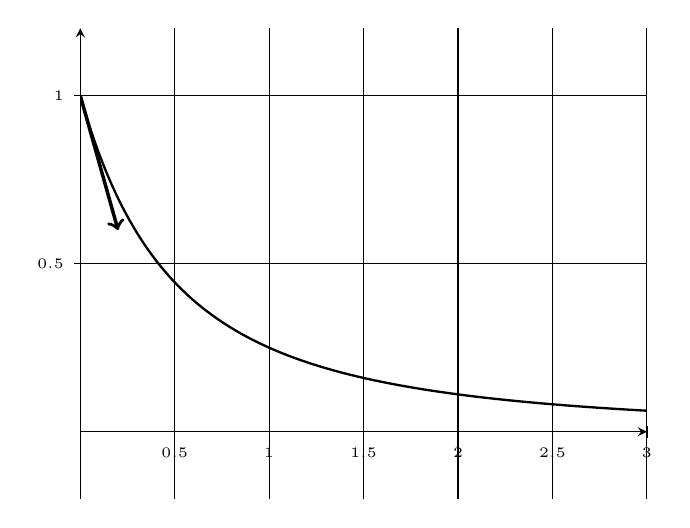
\begin{tikzpicture}[xscale=1.5, yscale = 1.5, scale = .7, transform
      shape, %
      declare function = { %
        g(\x) = 1/(1+\x)^2; %
        h(\x) = -2*\x+1; %
      },] %
      \pgfplotsset{every tick label/.append style={font=\tiny}}
      \begin{axis}[%
        xmin = 0, %
        xmax = 3, %
        ymin = -0.2, %
        ymax = 1.2, %
        no markers, %
        axis x line = center, %
        axis y line = center, %
        grid = both, %
        % xticklabels={},
        % ytick={-2,-1,0,1,2,3,4},%
        % yticklabels={-2,-1,0,1,2,3,4}%
        ] %
        \xdef\epsi{0.2}; %
        \addplot[samples=150, domain=0:3, blue, thick] {g(x)}; %
        \addplot[->, samples=2, domain={0}:{\epsi}, red, very 
	thick]{h(x)}; %
      \end{axis}
    \end{tikzpicture}
    \end{center}~\\[-1.4cm]
 \end{noliste}
\end{proof}



\newpage



\item Pour $n \geq 1$, justifier que $g_n$ est dérivable sur
  $[0,+\infty[$ et montrer que~:
  \[ 
  \forall x \in [0,+\infty[, \ g_n'(x) \geq 0 \ \Leftrightarrow \ n
  \geq 2\ln(1+x)
  \]
  En déduire les variations de la fonction $g_n$ lorsque $n \geq 1$.\\ 
  Calculer soigneusement $\dlim{x \to + \infty} g_n(x)$.
  
  \begin{proof}~\\
    Soit $n\geq 1$.
    \begin{noliste}{$\sbullet$}
    \item La fonction $g_n$ est dérivable sur $[0,+\infty[$ car elle
      est le quotient de fonctions dérivables sur $[0,+\infty[$ dont
      le dénominateur ne s'annule pas ($\forall x \in [0,+\infty[$,
      $(1+x)^2 \neq 0$).
      
    \item Soit $x\in [0,+ \infty[$.
      \[
      \begin{array}{rcl}
        g_n'(x) & = & \dfrac{n \, \dfrac{(\ln(1+x))^{n-1}}{\bcancel{1+x}} 
          \, (1+x)^{\bcancel{2}} - 2(1+x) \, 
          (\ln(1+x))^n}{(1+x)^4}
        \\[.6cm]
        & = & \dfrac{n \, (1+x) (\ln(1+x))^{n-1} -2(1+x)(\ln(1+x))^n}{(1+
          x)^7}
        \\[.6cm]
        & = & \dfrac{(1+x)(\ln(1+x))^{n-1} 
          \left(n -2\ln(1+x)\right)}{(1+x)^7}
      \end{array}
      \]
      Comme $x\geq 0$, on a :
      \[
      1+x \geq 1 \quad \mbox{ et } \quad \ln(1+x)\geq 0
      \]
      \conc{On obtient alors : $\forall x\in [0,+\infty[$,\\[.2cm]
        $g_n'(x)\geq 0 \ \Leftrightarrow \ n-2\ln(1+x) \geq 0
        \ \Leftrightarrow \ n \geq 2\ln(1+x)$.}
      
    \item Soit $x\in [0,+\infty[$.
      \[
      \begin{array}{rcl@{\quad}>{\it}R{5cm}}
        g_n'(x) \geq 0 & \Leftrightarrow & n \geq 2\ln(1+x)
        \ \Leftrightarrow \ \dfrac{n}{2} \geq \ln(1+x)
        \\[.2cm]
        & \Leftrightarrow & \ee^{\frac{n}{2}} \geq 1+x
        & (car $x\mapsto \ee^x$ est strictement croissante sur $\R$)
        \nl
        \nl[-.4cm]
        & \Leftrightarrow & \ee^{\frac{n}{2}}-1 \geq x
      \end{array}
      \]
      Or : $\dfrac{n}{2} \geq 0$. Donc, par croissance de $x\mapsto
      \ee^x$ : $\ee^{\frac{n}{2}} \geq \ee^0=1$ \ et \
      $\ee^{\frac{n}{2}}-1 \geq 0$.\\[.2cm]
      On obtient alors le tableau de variations suivant :
  
  \begin{center}
      \begin{tikzpicture}[scale=0.8, transform shape]
        \tkzTabInit[lgt=4,espcl=3] %
        { %
        $x$ /1, %
        Signe de $g_n'(x)$ /1, %
        Variations de $g_n$ /2
        } %
        {$0$, $\ee^{\frac{n}{2}}-1$, $+\infty$} %
        \tkzTabLine{ , + , z , - , } % 
        \tkzTabVar{-/$0$, +/$\left(\dfrac{n}{2\ee}\right)^n$ , 
	-/$0$} %
      \end{tikzpicture}
     \end{center}
     
   \item Détaillons les éléments de ce tableau.
     \begin{noliste}{-}
     \item Tout d'abord : 
       \[
       g_n\left(\ee^{\frac{n}{2}}-1\right) =
       \dfrac{\left(\ln\left(\bcancel{1} +
             \ee^{\frac{n}{2}}-\bcancel{1}\right)\right)^n}
       {\left(\bcancel{1}+\ee^{\frac{n}{2}}-\bcancel{1}\right)^2} =
       \dfrac{\left(\ln\left(\ee^{\frac{n}{2}} \right)\right)^n}
       {\left(\ee^{\frac{n}{2}}\right)^2} =
       \dfrac{\left(\frac{n}{2}\right)^n}{\ee^{\bcancel{2}\,
           \frac{n}{\bcancel{2}}}} = \left(\dfrac{n}{2}\right)^n
       \dfrac{1}{\ee^n} =\left(\dfrac{n}{2\ee}\right)^n
       \]
       
    
       \newpage
    
    
    \item Et :
    \[
     g_n(0) = \dfrac{\left(\ln(1+0)\right)^n}{(1+0)^2}
     = \dfrac{\left(\ln(1)\right)^n}{1^2}=0
    \]
    
  \item Enfin : $\dlim{x\to+\infty} (1+x)=+\infty$.\\[.2cm]
    Et : $\dlim{y\to +\infty} \dfrac{(\ln(y))^n}{y^2}=0$, par
    croissances comparées. %
    \conc{Finalement, par composition de fonctions, $\dlim{x\to
        +\infty} g_n(x)=0$.}
  \end{noliste}
 \end{noliste}
 \begin{remarkL}{.75}
   Le calcul de $g_n\left(\ee^{\frac{n}{2}}-1\right)$ n'était pas
   indispensable dans cette question.
 \end{remarkL}~\\[-1.4cm]
\end{proof}


\item Montrer que, pour $n \geq 1$, $g_n$ admet un maximum sur 
$[0,+\infty[$ qui vaut~:
\[ 
M_n = \left( \dfrac{n}{2 \ee} \right)^n 
\]
et déterminer $\dlim{n \to + \infty} M_n$.

\begin{proof}~\\
 Soit $n\geq 1$.
 \begin{noliste}{$\sbullet$}
  \item La fonction $g_n$ est :
  \begin{noliste}{$\stimes$}
    \item croissante sur l'intervalle $\left[0, \ee^{\frac{n}{2}}-1
    \right]$,
    \item décroissante sur l'intervalle $\left[ \ee^{\frac{n}{2}} -1,
    +\infty \right[$.
  \end{noliste}
  \conc{Sur $[0,+\infty[$, La fonction $g_n$ admet un maximum $M_n$ en 
  $\ee^{\frac{n}{2}}-1$ et,\\[.2cm]
  d'après la question \itbf{1.b)}, $M_n=\left(\dfrac{n}{2\ee}\right)^n$}
  
  \begin{remark}
   Bien sûr, si le calcul de $g_n\left(\ee^{\frac{n}{2}}-1\right)$ 
   n'a pas été effectué à la question précédente, il est 
   obligatoire ici.
  \end{remark}

  
  \item On remarque :
  \[
   M_n = \left(\dfrac{n}{2\ee}\right)^n =
   \exp \left(n \ln \left(\dfrac{n}{2\ee}\right)\right)
  \]
  Or : $\dlim{n\to+\infty} n \ln\left(\dfrac{n}{2\ee}\right)=+\infty$. 
  Donc $\dlim{n\to + \infty} \exp \left(n \ln 
  \left(\dfrac{n}{2\ee}\right)\right) = +\infty$.
  \conc{$\dlim{n\to +\infty} M_n=+\infty$}~\\[-1.2cm]
 \end{noliste}
\end{proof}


\newpage


\item Montrer enfin que pour tout $n \geq 1$~:
  \[
  g_n(x)  = \oox{+\infty} \left( 
    \frac{1}{x^{\frac{3}{2}}} \right) 
  \]

  \begin{proof}~\\
    Soit $n\geq 1$.
    \begin{noliste}{$\sbullet$}
    \item Tout d'abord, pour tout $x\in [0,+\infty[$ :
      \[      
      \dfrac{g_n(x)}{\frac{1}{x^{\frac{3}{2}}}} \ = \ x^{\frac{3}{2}}
      \ g_n(x) \ = \ x^{\frac{3}{2}} \dfrac{(\ln(1+x))^n} {(1+x)^2}
      \]

    \item En posant $y = 1+x$, on a :
      \[
      x^{\frac{3}{2}} g_n(x) \ = \ x^{\frac{3}{2}}
      \dfrac{(\ln(1+x))^n} {(1+x)^2} \ = \ (y-1)^{\frac{3}{2}}
      \dfrac{(\ln(y))^n}{y^2}
      \]
      Or :
      \[
      (y-1)^{\frac{3}{2}} \dfrac{(\ln(y))^n}{y^2} \eq{y}{+\infty}
      y^{\frac{3}{2}} \dfrac{(\ln(y))^n}{y^2} =
      \dfrac{(\ln(y))^n}{y^{\frac{1}{2}}}
      \]
      De plus, par croissances comparées : $\dlim{y\to +\infty}
      \dfrac{(\ln(y))^n}{y^{\frac{1}{2}}} = 0$. Donc :
      $\dlim{y\to+\infty} (y-1)^{\frac{3}{2}} \dfrac{(\ln(y))^n}{y^2}
      =0$.

    \item Finalement :
      \begin{noliste}{$\stimes$}
      \item $\dlim{x\to +\infty} (1+x)=+\infty$,
      \item $\dlim{y\to+\infty} (y-1)^{\frac{3}{2}}
        \dfrac{(\ln(y))^n}{y^2} =0$.
      \end{noliste}
      On en déduit, par composition de fonctions : $\dlim{x\to+\infty}
      x^{\frac{3}{2}} g_n(x)=0$.
    \end{noliste}

 \conc{$\forall n\geq 1$, $g_n(x)=\oox{+\infty} \left(
 \dfrac{1}{x^{\frac{3}{2}}}\right)$}~\\[-1cm]
\end{proof}
\end{noliste}


\item On pose pour tout $n \in \N$~:
\[ 
I_n = \dint{0}{+\infty} g_n(t) dt 
\]
\begin{noliste}{a)}
\item Montrer que l'intégrale $I_0$ est convergente et la calculer.

\begin{proof}~
 \[
  I_0=\dint{0}{+\infty} g_0(t)\dt
 \]
 \begin{noliste}{$\sbullet$}
  \item La fonction $g_0$ est continue sur $[0,+\infty[$.
  
  \item Soit $A \in [0,+\infty[$.
  \[
   \dint{0}{A} g_0(t) \dt =
   \dint{0}{A} \dfrac{1}{(1+t)^2} \dt = \Prim{-\dfrac{1}{1+t}}{0}{A}
   =-\dfrac{1}{1+A} +1
  \]
  Or $\dlim{A\to+\infty} \dfrac{1}{1+A} =0$.
  \conc{Donc l'intégrale $I_0$ converge et vaut $1$.}
  
  \begin{remark}
   L'énoncé demande ici de démontrer la convergence de $I_0$ 
   \texttt{ET} de calculer sa valeur.\\
   Dans ce cas, on se lancera directement dans le calcul de l'intégrale.
  \end{remark}~\\[-1.4cm]
 \end{noliste}
\end{proof}


\newpage


\item Montrer que pour tout entier $n \geq 1$, l'intégrale $I_n$ 
est convergente.

\begin{proof}~\\
Soit $n\geq 1$.
 \begin{noliste}{$\sbullet$}
  \item La fonction $g_n$ est continue sur $[0,+\infty[$.
  
  \item
  \begin{noliste}{$\stimes$}
    \item $g_n(x) = \oox{+\infty} 
    \left(\dfrac{1}{x^{\frac{3}{2}}}\right)$
    \item $\forall x \in [1,+\infty[$, $g_n(x)\geq 0$ et 
    $\dfrac{1}{x^{\frac{3}{2}}}\geq 0$
    \item L'intégrale $\dint{1}{+\infty} \dfrac{1}{x^{\frac{3}{2}}}\dx$ 
    est une intégrale de Riemann impropre en $+\infty$, d'exposant 
    $\dfrac{3}{2}$, donc elle converge.
  \end{noliste}
  Par critère de négligeabilité des intégrales généralisées de 
  fonctions continues positives, l'intégrale
  $\dint{1}{+\infty} g_n(x) \dx$ converge.
  
  \item De plus, $g_n$ est continue sur le segment $[0,1]$. Donc 
  l'intégrale $\dint{0}{1} g_n(x) \dx$ est bien définie.
 \end{noliste}
 \conc{Finalement, pour tout $n\geq 1$, $I_n = \dint{0}{+\infty}
 g_n(x) \dx$ converge.}
 \begin{remark}
  Il est encore une fois important de bien lire la question : 
  l'énoncé demande cette fois simplement de montrer la 
  convergence de $I_n$ (sans la calculer).\\
  Dans ce cas, on pensera en priorité à l'utilisation 
  d'une critère de comparaison / équivalence / négligeabilité.
 \end{remark}~\\[-1.4cm]
\end{proof}


\item À l'aide d'une intégration par parties, montrer que~:
\[ 
\forall n \in \N, \ I_{n+1} = (n+1) I_n 
\]

\begin{proof}~\\
  Soit $A\geq 0$. On effectue une intégration par parties (IPP).
  \[
  \renewcommand{\arraystretch}{2.2}
  \begin{array}{|rcl@{\qquad}rcl}
   u(x) & = & (\ln(1+x))^{n+1} & u'(x) & = & (n+1) 
   \dfrac{(\ln(1+x))^n}{1+x} \\
   v'(x) & = & \dfrac{1}{(1+x)^2} & v(x) & = & -\dfrac{1}{1+x}
  \end{array}
  \]
Cette IPP est valide car les fonctions $u$ et $v$ sont de classe 
$\Cont{1}$ sur $[0,A]$. On obtient :
\[
 \begin{array}{rcl}
  \dint{0}{A} g_{n+1}(x) \dx & = & \dint{0}{A} \dfrac{(\ln(1+x))^n}
  {(1+x)^2} \dx 
  \\[.6cm]
  & = & \Prim{-\dfrac{(\ln(1+x))^{n+1}}{1+x}}{0}{A} + (n+1)
   \dint{0}{A}\dfrac{(\ln(1+x))^n}{(1+x)^2} \dx
   \\[.6cm]
   & = & -\dfrac{(\ln(1+A))^{n+1}}{1+A} + (n+1) \dint{0}{A} 
   \dfrac{(\ln(1+x))^n}{(1+x)^2} \dx
   \\[.6cm]
   & = & -\dfrac{(\ln(1+A))^{n+1}}{1+A} + (n+1) \dint{0}{A} 
   g_n(x) \dx
 \end{array}
\]


\newpage


Or, par croissances comparées : $\dlim{A\to+\infty} 
\dfrac{(\ln(1+A))^{n+1}}{1+A} = 0$.\\[.2cm]
De plus l'intégrale $I_n$ converge d'après la question \itbf{2.b)}. 
D'où :
\[
 \dint{0}{+\infty} g_{n+1}(x) \dx = 0+(n+1) \dint{0}{+\infty} 
 g_n(x) \dx
\]
\conc{On en déduit : $\forall n\in\N^*$, $I_{n+1}=(n+1)I_n$.}~\\[-1.2cm]
\end{proof}

\item En déduire que~:
  \[ 
  \forall n \in \N, \ I_n = n! 
  \]

\begin{proof}~\\
 Démontrons par récurrence : $\forall n\in\N$, $\PP{n}$ \quad 
 où \quad $\PP{n}$ : $I_n=n!$.
 \begin{noliste}{\fitem}
 \item {\bf Initialisation} : \\
   D'après la question \itbf{2.a)},
   $I_0=1=0!$.\\
   D'où $\PP{0}$.
  
  \item {\bf Hérédité} : soit $n\in\N$.\\
  Supposons $\PP{n}$ et démontrons $\PP{n+1}$ (c'est-à-dire :
  $I_{n+1}=(n+1)!$).
  \[
   \begin{array}{rcl@{\quad}>{\it}R{5cm}}
    I_{n+1} & = & (n+1) I_n & (d'après la question \itbf{2.c)}
    \nl
    \nl[-.4cm]
    & = & (n+1) \times n! & (par hypothèse de récurrence)
    \nl
    \nl[-.4cm]
    & = & (n+1)!
   \end{array}
  \]
  D'où $\PP{n+1}$.
\end{noliste}
\conc{Ainsi, par principe récurrence : $\forall n\in\N$, $I_n=n!$}~\\[-1.2cm]
\end{proof}
\end{noliste}

\item Pour tout $n \in \N$, on définit la fonction $f_n$ par~:
\[ 
\forall x \in \R, \ f_n(x) = \left\{ 
\begin{array}{cl} 
0 & \text{ si } x < 0 \\[.2cm] 
\dfrac{1}{n!} \ g_n(x) & \text{ si } 
x \geq 0 \end{array} \right. 
\]
\begin{noliste}{a)}
\item Montrer que pour tout $n \in \N$, $f_n$ est une densité de
  probabilité.

  \begin{proof}~\\
    Soit $n\in\N$.
    \begin{noliste}{$\sbullet$}
    \item Soit $x\in\R$. Deux cas se présentent.
      \begin{noliste}{$\stimes$}
      \item Si $x<0$ : $f_n(x)=0$. Donc : $f_n(x) \geq 0$.
      \item Si $x\geq 0$. D'après le tableau de variations dressé en 
        question \itbf{1.b)}, on a : $f_n(x)=\dfrac{1}{n!} g_n(x) \geq 0$.
      \end{noliste}
      \conc{D'où : $\forall x\in\R$, $f_n(x) \geq 0$.}
      
    \item 
      \begin{noliste}{$\stimes$}
      \item La fonction $f_n$ est continue sur $]-\infty, 0[$ car elle
        est constante sur cet intervalle.
      \item La fonction $f_n$ est continue sur $]0,+\infty[$ car la
        fonction $g_n$ l'est.
      \end{noliste}
      \conc{Ainsi $f_n$ est continue sur $\R$ sauf éventuellement en $0$.}  
      \begin{remark}
        La continuité sur $\R$ sauf en un nombre fini de points suffit 
        ici. Mais rien n'interdit d'utiliser l'étude de $g_n$ pour 
        conclure quant à la continuité de $f_n$ en $0$.
      \end{remark}
  

  \newpage

  
  \item Montrons que $\dint{-\infty}{+\infty} f_n(t) \dt$ converge 
  et vaut $1$.\\[.2cm]
  Tout d'abord : $\dint{-\infty}{+\infty} f_n(t) \dt=
  \dint{0}{+\infty} f_n(t) \dt$, car $f_n$ est nulle en dehors de 
  $[0, +\infty[$.\\[.2cm]
  De plus, comme l'intégrale $\dint{0}{+\infty} g_n(t) \dt$
  converge :
  \[
   \begin{array}{rcl@{\quad}>{\it}R{3cm}}
    \dint{0}{+\infty} f_n(t) \dt & = & \dint{0}{+\infty} \dfrac{1}{n!}
    g_n(t) \dt \ = \ \dfrac{1}{n!} \dint{0}{+\infty} g_n(t) \dt
    \\[.6cm]
    & = & \dfrac{1}{n!} \, I_n \ = \ \dfrac{1}{\bcancel{n!}} \,
    \bcancel{n!} & (d'après la question \itbf{2.d)})
    \nl
    \nl[-.4cm]
    & = & 1
   \end{array}
  \]
  \conc{Ainsi : $\dint{-\infty}{+\infty} f_n(t) \dt $ converge et vaut 
  $1$.}
 \end{noliste}
 Finalement, on a montré  :
 \begin{noliste}{-}
  \item $\forall x\in \R$, $f_n(x) \geq 0$,
  \item $f_n$ est continue sur $\R$, sauf éventuellement en $0$,
  \item L'intégrale $\dint{-\infty}{+\infty} f_n(t) \dt$ converge et
    vaut $1$.
 \end{noliste}
 \conc{Pour tout $n\in\N$, $f_n$ est une densité de
   probabilité.}~\\[-1.2cm]
\end{proof}
\end{noliste}

\noindent \hspace{-0.5cm} On considère à présent, pour tout $n \in 
\N$, $X_n$ une variable aléatoire réelle admettant $f_n$ pour 
densité.

\noindent \hspace{-0.5cm} On notera $F_n$ la fonction de répartition de 
$X_n$.

\begin{noliste}{a)}
\setcounter{enumii}{1}
\item La variable aléatoire $X_n$ admet-elle une espérance~?

\begin{proof}~
 \begin{noliste}{$\sbullet$}
 \item La \var $X_n$ admet une espérance si et seulement si
   l'intégrale impropre $\dint{-\infty}{+\infty} t \, f_n(t) \dt$ est
   absolument convergente, ce qui équivaut à démontrer la convergence
   pour les calculs de moments du type $\dint{-\infty}{+\infty} t^m \,
   f_n(t) \dt$.
  
  \item La fonction $f_n$ est nulle en dehors de $[0,+\infty[$, donc : 
  \[
   \dint{-\infty}{+\infty} t \, f_n(t) \dt = 
   \dint{0}{+\infty} t \, f_n(t) \dt
  \]
  
\item
  \begin{noliste}{$\stimes$}
  \item Démontrons : $\dfrac{1}{t} = \oo{t}{+\infty} \left( t\, f_n(t)
    \right)$.
    \[
     \dfrac{\frac{1}{t}}{t\, f_n(t)} =
     \dfrac{\frac{1}{t}}{t\, g_n(t)}= \dfrac{(1+t)^2}{t^2 \, 
     (\ln(1+t))^n} \eq{t}{+\infty} \dfrac{\bcancel{t^2}}
     {\bcancel{t^2} \, (\ln(1+t))^n} = \dfrac{1}{(\ln(1+t))^n}
    \]
    Or : $\dlim{t\to +\infty} \dfrac{1}{(\ln(1+t))^n} =0$. Donc :
    $\dlim{t\to+\infty} \dfrac{\frac{1}{t}}{t\, f_n(t)}=0$.\\[.2cm]
    Ainsi : $\dfrac{1}{t} = \oo{t}{+\infty} (t\, f_n(t))$.


    \newpage


  \item Pour tout $t\in [1,+\infty[$ : $t\, f_n(t) \geq 0$ et
    $\dfrac{1}{t} \geq 0$.
    
    \item L'intégrale $\dint{1}{+\infty} \dfrac{1}{t} \dt$ est une 
    intégrale de Riemann impropre en $+\infty$, d'exposant $1$, donc 
    elle diverge.
  \end{noliste}
  Par critère de négligeabilité des intégrales généralisées de
  fonctions continues positives, l'intégrale $\dint{1}{+\infty} t\,
  f_n(t) \dt$ diverge.\\[.2cm]
  Ainsi $\dint{-\infty}{+\infty} t \, f_n(t) \dt$ diverge.
  \conc{$X_n$ n'admet pas d'espérance.}
 \end{noliste}

 
 \begin{remark}
  Il y a plusieurs réflexes à acquérir pour ce type de questions :
  \begin{noliste}{1)}
    \item l'énoncé demande de déterminer l'existence de $\E(X_n)$
    \texttt{UNIQUEMENT}, donc on privilégiera l'utilisation d'un 
    critère de comparaison / équivalence / négligeabilité.
    
  \item l'énoncé ne demande pas \og Montrer que $X_n$ admet une
    espérance \fg{}, mais \og $X_n$ admet-elle une espérance ? \fg{}.
    Il y a donc de fortes chances que la réponse attendue soit \og
    $X_n$ \texttt{N}'admet \texttt{PAS} d'espérance \fg{}. C'est
    pourquoi on cherche ici à montrer en priorité $\dfrac{1}{t} =
    \oo{t}{+\infty} \left(t \, f_n(t)\right)$ plutôt que $t \, f_n(t)
    = \oo{t}{+\infty} \left(\dfrac{1}{t^\alpha}\right)$ avec $\alpha
    >1$.
  \end{noliste}
 \end{remark}~\\[-1.4cm]
\end{proof}


\item Que vaut $F_n(x)$ pour $x < 0$ et $n \in \N$~?

  \begin{proof}~\\
    Soit $n\in\N$. Soit $x<0$.
    \[
    F_n(x)= \Prob(\Ev{X_n\leq x}) = \dint{-\infty}{x} f_n(t) \dt
    = 0 \quad \mbox{\it{(car : $\forall t<0$, $f_n(t)=0$)}}
    \]
    \conc{$\forall n\in\N$, $\forall x<0$, $F_n(x)=0$}~\\[-1cm]
  \end{proof}
  
\item Calculer $F_0(x)$ pour $x \geq 0$.
  
  \begin{proof}~\\
    Soit $x\geq 0$.
    \[
    \begin{array}{rcl@{\quad}>{\it}R{3cm}}
      F_0(x) & = & \Prob(\Ev{X_0\leq x}) \ = \ \dint{-\infty}{x} f_0(t)\dt
      \\[.6cm]
      & = & \dint{0}{x} \dfrac{1}{0!} \, g_0(t) \dt & (car $x\geq 0$)
      \nl
      \nl[-.2cm]
      & = & \dint{0}{x} \dfrac{1}{(1+t)^2} \dt \ = \ 
      \Prim{-\dfrac{1}{1+t}}{0}{x}
      \\[.6cm]
      & = & 1-\dfrac{1}{1+x}
    \end{array}
    \]
    \conc{Finalement : $\forall x\geq 0$, $F_0(x) = 
      1-\dfrac{1}{1+x}$}~\\[-.8cm]
  \end{proof}


\newpage


\item Soit $x \geq 0$ et $k \in \N^*$. Montrer que~:
  \[ 
  F_k(x) - F_{k-1}(x) = - \dfrac{1}{k!} \dfrac{(\ln(1+x))^k}{1+x} 
  \]

\begin{proof}~
 \[
  \begin{array}{rcl@{\quad}>{\it}R{3cm}}
   F_k(x) & = & \Prob(\Ev{X_k\leq x}) \ = \ \dint{0}{+\infty} f_k(t) \dt
   \\[.6cm]
   & = & \dint{0}{x} \dfrac{1}{k!} g_k(t) \dt & (car $x\geq 0$)
   \nl
   \nl[-.2cm]
   & = & \dfrac{1}{k!} \dint{0}{x} \dfrac{(\ln(1+t))^k}{(1+t)^2} \dt
  \end{array}
 \]
 On effectue une intégration par parties (IPP).
 \[
  \renewcommand{\arraystretch}{2.2}
  \begin{array}{|rcl@{\qquad}rcl}
   u(t) & = & (\ln(1+t))^{k} & u'(t) & = & k 
   \dfrac{(\ln(1+t))^{k-1}}{1+t} \\
   v'(t) & = & \dfrac{1}{(1+t)^2} & v(t) & = & -\dfrac{1}{1+t}
  \end{array}
 \]
 Cette IPP est valide car $u$ et $v$ sont de classe $\Cont{1}$ sur
 $[0,x]$.
 \[
  \begin{array}{rcl}
   F_k(x) & = & \dfrac{1}{k!} \left(\Prim{-\dfrac{(\ln(1+t))^k}{1+t}}{0}
   {x} + k \dint{0}{x} \dfrac{(\ln(1+t))^{k-1}}{(1+t)^2} \dt\right)
   \\[.6cm]
   & = & -\dfrac{1}{k!} \dfrac{(\ln(1+x))^k}{1+x} + \dfrac{k}{k!}
   \dint{0}{x} \dfrac{(\ln(1+t))^{k-1}}{(1+t)^2} \dt
   \\[.6cm]
   & = & -\dfrac{1}{k!} \dfrac{(\ln(1+x))^k}{1+x} + \dfrac{1}{(k-1)!}
   \dint{0}{x} \dfrac{(\ln(1+t))^{k-1}}{(1+t)^2} \dt
   \\[.6cm]
   & = & -\dfrac{1}{k!} \dfrac{(\ln(1+x))^k}{1+x} +
   \dint{0}{x} f_{k-1}(t)\dt 
   \\[.6cm]
   & = & -\dfrac{1}{k!} \dfrac{(\ln(1+x))^k}{1+x} + F_{k-1}(x)
  \end{array}
 \]
 \conc{$\forall k\in\N^*$, $\forall x>0$, 
 $F_k(x)-F_{k-1}(x) = -\dfrac{1}{k!} 
 \dfrac{(\ln(1+x))^k}{1+x}$}~\\[-1cm]
\end{proof}


\item En déduire une expression de $F_n(x)$ pour $x \geq 0$ et $n 
\in \N^*$ faisant intervenir une somme (on ne cherchera pas à 
calculer cette somme).

\begin{proof}~\\
 Soit $n\in\N^*$. Soit $x\geq 0$.
 \begin{noliste}{$\sbullet$}
  \item D'après la question précédente :
  \[
   \forall k\in\N^*, \ F_k(x)-F_{k-1}(x) = -\dfrac{1}{k!} 
   \dfrac{(\ln(1+x))^k}{1+x}
  \]
  
  \item On somme alors ces égalités pour $k$ variant de $0$ à $n$. On 
  obtient :
  \[
   \Sum{k=1}{n} (F_k(x) - F_{k-1}(x)) = \Sum{k=1}{n} \left(
   -\dfrac{1}{k!} \dfrac{(\ln(1+x))^k}{1+x}\right)
   =-\dfrac{1}{1+x} \, \Sum{k=1}{n} \dfrac{(\ln(1+x))^k}{k!}
  \]
  
  
  \newpage
  
  
  Par télescopage, on a alors :
  \[
   F_n(x) - F_0(x) = -\dfrac{1}{1+x} \, \Sum{k=1}{n} 
   \dfrac{(\ln(1+x))^k}{k!}
  \]
  
  \item Or, d'après la question \itbf{3.d)} : $F_0(x)=1-\dfrac{1}{1+x}$.
  Donc :
  \[
   \begin{array}{rcl@{\quad}>{\it}R{4cm}}
    F_n(x) & = & F_0(x) -\dfrac{1}{1+x} \, \Sum{k=1}{n} 
    \dfrac{(\ln(1+x))^k}{k!}
    \\[.6cm]
    & = & 1-\dfrac{1}{1+x} -\dfrac{1}{1+x} \, \Sum{k=1}{n} 
    \dfrac{(\ln(1+x))^k}{k!}
    \\[.6cm]
    & = & 1 -\dfrac{1}{1+x} \, \Sum{k=0}{n} 
    \dfrac{(\ln(1+x))^k}{k!}
    & (car : $\dfrac{(\ln(1+x))^0}{0!}=1$)
   \end{array}
  \]
  \conc{Finalement : $\forall n\in\N^*$, $\forall x\geq 0$, 
  $F_n(x) = 1 -\dfrac{1}{1+x} \, \Sum{k=0}{n} 
    \dfrac{(\ln(1+x))^k}{k!}$}~\\[-1.2cm]
 \end{noliste}
\end{proof}


\item Pour $x \in \R$ fixé, déterminer la limite de $F_n(x)$  
lorsque $n$ tend vers $+\infty$.

\begin{proof}~\\
  Soit $x\in\R$. Deux cas se présentent.
 \begin{noliste}{$\sbullet$}
  \item \dashuline{Si $x<0$}, alors : $F_n(x)=0$. Donc 
  $\dlim{n\to+\infty} F_n(x)=0$.
  
\item \dashuline{Si $x\geq 0$}, alors : $F_n(x) = 1 -\dfrac{1}{1+x}
  \, \Sum{k=0}{n} \dfrac{(\ln(1+x))^k}{k!}$.\\[.2cm]
  Or $\Sum{n\geq 0}{} \dfrac{(\ln(1+x))^k}{k!}$ est la série
  exponentielle de paramètre $\ln(1+x)$.\\[.2cm]
  Elle est donc convergente et :
  \[
   \Sum{k=0}{+\infty} \dfrac{(\ln(1+x))^k}{k!} = 
   \exp\left(\ln(1+x)\right) = 1+x
  \]
  Ainsi la suite $(F_n(x))_{n\geq 1}$ converge et on obtient :
  \[
   \dlim{n\to+\infty} F_n(x)=1-\dfrac{1}{\bcancel{1+x}}\, 
   \bcancel{(1+x)} = 1-1=0
  \]
 \end{noliste}
 \conc{Finalement : $\forall x\in\R$, $\dlim{n\to+\infty}
   F_n(x) = 0$.}~\\[-1cm]
\end{proof}


\item La suite de variables aléatoires $(X_n)_{n \in \N}$ 
converge-t-elle en loi~?

\begin{proof}~\\
 Raisonnons par l'absurde et supposons qu'il existe une \var
  $X$ de fonction de répartition $G$ telle que $(X_n)$ converge en 
  loi vers $X$.\\
  Alors, pour tout $x\in\R$ où $G$ est continue, on a :
  \[
   \dlim{n\to+\infty} F_n(x) = G(x)
  \]
  
  
  
  \newpage
  
  
  
  Or, d'après la question précédente : 
  $\forall x\in\R$, $\dlim{n\to+\infty} F_n(x)=0$. Donc : 
  $\forall x\in\R$, $G(x)=0$.\\[.2cm]
  Ceci est absurde car $G$ est une fonction de répartition, donc, en 
  particulier, $\dlim{x\to+\infty} G(x)=1$.
  
  \conc{La suite $(X_n)$ ne converge pas en loi.}
  
  \begin{remarkL}{.8}
    Il convient d'insister ici sur la définition de la convergence en loi.\\
    $(X_n)$ converge en loi vers $X$ si, pour tout $x\in\R$ où $F_X$
    est continue, on a :
   \[
    \dlim{n\to+\infty} F_{X_n}(x) = F_X(x)
   \]
   En particulier :
   \begin{noliste}{1)}
   \item cette convergence n'a pas besoin d'être vraie pour tout
     $x\in\R$. \\
     Elle peut ne pas être vérifiée pour les points de discontinuité
     de $F_X$.
    \item on s'intéresse bien ici aux points de continuité de $F_X$ 
    et non de $F_{X_n}$.
   \end{noliste}
  \end{remarkL}~\\[-1.4cm]
\end{proof}

\end{noliste}

\item Pour tout $n \in \N$, on note $Y_n = \ln(1+X_n)$.
\begin{noliste}{a)}
\item Justifier que $Y_n$ est bien définie. Quelles sont les valeurs 
prises par $Y_n$~?

\begin{proof}~
 \begin{noliste}{$\sbullet$}
  \item Sans perte de généralité, on considère pour la suite que : 
  $X_n(\Omega) = [0,+\infty[$.\\ 
  Donc $\ln(1+X_n)$ est bien définie.
  \conc{Ainsi, $Y_n$ est bien définie.}
  
  \item Déterminons $Y_n(\Omega)$, où $Y_n = h(X_n)$ avec $h:x \mapsto 
  \ln(1+x)$.\\[.1cm]
  Comme précisé précédemment : $X_n(\Omega) = [0,+\infty[$.
  On en déduit :
  \[
   \begin{array}{rcl@{\quad}>{\it}R{6cm}}
    Y_n(\Omega) &=& h(X_n)(\Omega) \ = \ h(X_n(\Omega))
    \\[.2cm]
    & = & h([0,+\infty[)
    \\[.2cm]
    & = & [ h(0), \dlim{x\to +\infty} h(x) [
    & (car $h$ est continue et strictement croissante sur $[0,
    +\infty[$)
    \nl
    \nl[-.2cm]
    & = & [0,+\infty[ & (car $h(0)=0$ et $\dlim{x\to +\infty}
    h(x) = +\infty$)
   \end{array}
  \]
  \conc{Ainsi : $Y_n(\Omega) = [0,+\infty[$}~\\[-1.2cm]
 \end{noliste}
\end{proof}



\item Justifier que $Y_n$ admet une espérance et la calculer.

\begin{proof}~
 \begin{noliste}{$\sbullet$}
 \item La fonction $f_n$ est nulle en dehors de $[0,+\infty[$.\\[.1cm]
   Ainsi, d'après le théorème de transfert, la \var $Y_n= \ln(1+X_n)$
   admet une espérance si et seulement si l'intégrale impropre
   $\dint{0}{+\infty} \ln(1+t) f_n(t) \dt$ est absolument convergente,
   ce qui équivaut à démontrer sa convergence car l'intégrande est
   positive :
   \[
   \forall t \in [0,+\infty[, \ \ln(1+t) \ f_n(t) \geq 0
   \]

  
  \newpage
  
  
  \item Soit $t \in [0,+\infty[$.
  \[
   \begin{array}{rcl@{\quad}>{\it}R{4.5cm}}
    \ln(1+t) f_n(t) & = & 
    \ln(1+t) \dfrac{1}{n!} \dfrac{(\ln(1+t))^n}
    {(1+t)^2} & (par définition de $f_n$)
    \nl
    \nl[-.2cm]
    & = & \dfrac{1}{n!} \dfrac{(\ln(1+t))^{n+1}}
    {(1+t)^2}
    \\[.6cm]
    & = & (n+1) \dfrac{1}{(n+1)!} 
    \dfrac{(\ln(1+t))^{n+1}}{(1+t)^2}
    \\[.6cm]
    & = & (n+1) f_{n+1}(t)  
    & (par définition de $f_{n+1}$)
   \end{array}
  \]
  
\item Or la fonction $f_{n+1}$ est une densité nulle en dehors de
  $[0,+\infty[$. \\
  Donc l'intégrale $\dint{0}{+\infty} f_{n+1}(t) \dt$
  converge et vaut $1$.\\
  On en déduit que l'intégrale $\dint{0}{+\infty} \ln(1+t) f_n(t) \dt$
  converge et :
  \[
   \dint{0}{+\infty} \ln(1+t) f_n(t) \dt = (n+1) \times 1 =
   (n+1)
  \]
 \end{noliste}
 \conc{On en déduit que $Y_n$ admet une espérance et $\E(Y_n) = n+1$.}
 
 \begin{remark}
  On rappelle l'énoncé du théorème de transfert pour les \var à densité 
  :\\
  Soit $X$ une \var de densité $f$ nulle en dehors d'un intervalle 
  $]a,b[$, et $g$ une fonction {\bf 
  continue} sur $]a,b[$ sauf éventuellement en un nombre fini de 
  points.\\ 
  Si l'intégrale $\dint{a}{b} g(t) \, f(t) \dt$ 
  est {\bf absolument convergente}, alors la \var $g(X)$ admet une 
  espérance et on a :
  \[
   \E(g(X)) = \dint{a}{b} g(t) \, f(t) \dt
  \]
  On applique donc ici le théorème de transfert pour la fonction 
  $g:t\mapsto \ln(1+t)$.
 \end{remark}~\\[-1.4cm]
\end{proof}


\item Justifier que $Y_n$ admet une variance et la calculer.

  \begin{proof}~
    \begin{noliste}{$\sbullet$}
    \item La fonction $f_n$ est nulle en dehors de $[0,+\infty[$.\\[.1cm]
      Donc, d'après le théorème de transfert, la \var $Y_n =
      \ln(1+X_n)$ admet une espérance si et seulement si l'intégrale
      impropre $\dint{0}{+\infty} (\ln(1+t))^2 f_n(t) \dt$ est
      absolument convergente, ce qui équivaut à démontrer sa
      convergence puisque l'intégrande est positive :
      \[
      \forall t \in [0,+\infty[, \ (\ln(1+t))^2 f_n(t) \geq 0
      \]
      % Donc démontrer que l'intégrale $\dint{0}{+\infty} (\ln(1+t))^2
      % f_n(t) \dt$ converge absolument équivaut à démontrer qu'elle
      % converge.
      
  
      \newpage
  
  
  \item Soit $t \in [0,+\infty[$.
  \[
   \begin{array}{rcl@{\quad}>{\it}R{5cm}}
    (\ln(1+t))^2 f_n(t)
    & = & 
    (\ln(1+t))^2 \dfrac{1}{n!} \dfrac{(\ln(1+t))^n}
    {(1+t)^2} & (par définition de $f_n$)
    \nl
    \nl[-.2cm]
    & = & \dfrac{1}{n!} \dfrac{(\ln(1+t))^{n+2}}
    {(1+t)^2} 
    \\[.6cm]
    & = & (n+2)(n+1) \dfrac{1}{(n+2)!} 
    \dfrac{(\ln(1+t))^{n+2}}{(1+t)^2}
    \\[.6cm]
    & = & (n+2)(n+1) f_{n+2}(t)
    & (par définition de $f_{n+2}$)
   \end{array}
  \]
  
  \item Or la fonction $f_{n+2}$ est une densité nulle en dehors de 
  $[0,+\infty[$. \\
  Donc l'intégrale $\dint{0}{+\infty} f_{n+2}(t) \dt$
  converge et vaut $1$.\\
  On en déduit que l'intégrale $\dint{0}{+\infty} (\ln(1+t))^2 f_n(t) 
  \dt$ converge et :
  \[
   \dint{0}{+\infty} (\ln(1+t))^2 f_n(t) \dt = (n+1)(n+2) \times 1 =
   (n+1)(n+2)
  \]
  \conc{Ainsi $Y_n$ admet un moment d'ordre $2$ et 
  $\E(Y_n^2)=(n+2)(n+1)$.}
  
  \item D'après la formule de K\oe{}nig-Huyghens :
  \[
   V(Y_n) = \E(Y_n^2)-(\E(Y_n))^2 = (n+2)(n+1)-(n+1)^2
   =(n+1)(\bcancel{n}+2-(\bcancel{n}+1)) = n+1
  \]
  \conc{On en déduit que $Y_n$ admet une variance et :
  $\V(Y_n)=n+1$.}
 \end{noliste}
 
 \begin{remark}
  On a, cette fois, appliqué le théorème de transfert avec la fonction 
  $g:t \mapsto (\ln(1+t))^2$.
 \end{remark}~\\[-1.4cm]
\end{proof}


\item On note $H_n$ la fonction de répartition de $Y_n$. Montrer que~:
\[ 
\forall x \in \R, \ H_n(x) = F_n(\ee^x-1) 
\]

\begin{proof}~\\
 Soit $x\in\R$.
 \[
  \begin{array}{rcl@{\quad}>{\it}R{5cm}}
   H_n(x) & = & \Prob(\Ev{Y_n \leq x}) \ = \ 
   \Prob(\Ev{\ln(1+X_n) \leq x})
   \\[.2cm]
   & = & \Prob(\Ev{1+X_n \leq \ee^x}) & (car $x\mapsto \ee^x$ est 
   strictement croissante sur $\R$)
   \nl
   \nl[-.4cm]
   & = & \Prob(\Ev{X_n \leq \ee^x-1}) \ = \ F_n(\ee^x-1)
  \end{array}
 \]
 \conc{Ainsi : $\forall x \in\R$, $H_n(x) = F_n(\ee^x-1)$}~\\[-1cm]
\end{proof}


\item Montrer que $Y_n$ est une variable aléatoire à densité et donner
  une densité de $Y_n$.

\begin{proof}~
 \begin{noliste}{$\sbullet$}
 \item Commençons par expliciter $H_n$.\\
   Soit $x \in \R$. Deux cas se présentent.
  \begin{noliste}{-}
    \item Soit $x<0$. Alors : $\ee^x-1 <0$. Donc, d'après la question 
    \itbf{4.d)}, on obtient :
    \[
     H_n(x) = F_n(\ee^x-1)=0
    \]
    
    
    \newpage
    
    
    \item Soit $x\geq 0$. Alors $\ee^x-1\geq 0$. Donc, toujours 
    d'après la question \itbf{4.d)}, on obtient :
    \[
     \begin{array}{rcl}
      H_n(x) & = & F_n(\ee^x-1)
      \\
      & = & 1 - \dfrac{1}{\bcancel{1}+\ee^x-\bcancel{1}}
      \ \Sum{k=0}{n} \dfrac{(\ln(\bcancel{1}+\ee^x-\bcancel{1}))^k}{k!}
      \\[.6cm]
      & = & 1-\dfrac{1}{\ee^x} \Sum{k=0}{n} \dfrac{(\ln(\ee^x))^k}{k!}
      \\[.6cm]
      & = & 1-\ee^{-x} \Sum{k=0}{n} \dfrac{x^k}{k!}
     \end{array}
    \]
  \end{noliste}
  \conc{Finalement : $\forall x \in\R$, $H_n(x)=\left\{
    \begin{array}{cl}
      0 & \mbox{ si $x<0$}\\
      1-\ee^{-x} \Sum{k=0}{n} \dfrac{x^k}{k!} & \mbox{ si $x\geq 0$}
    \end{array}
  \right.$.}%

\item Ainsi :
  \begin{noliste}{$\stimes$}
  \item $H_n$ est continue sur $]-\infty,0[$ car elle est constante
    sur cet intervalle.
    
  \item $H_n$ est continue sur $]0,+\infty[$ comme somme et produit de
    fonctions continues sur $]0,+\infty[$.
    
  \item d'une part : $\dlim{x \to 0^-} H_n(x)=0$.
    D'autre part : ~\\[-.2cm]
    \[
     \begin{array}{rcl@{\quad}>{\it}R{6cm}}
      \dlim{x\to0^+} H_n(x) & = & H_n(0) \ = \ 1-\ee^{-0} \Sum{k=0}{n} 
      \dfrac{0^k}{k!} 
      \\[.2cm]
      & = & 1 - 1 \ = \ 0 & (car $\forall x \in\R$, $\Sum{k=0}{n}
      \dfrac{x^k}{k!} = 1 + \Sum{k=1}{n} \dfrac{x^k}{k!}$)
      % \nl
      % \nl[-.4cm]
      % & = & 0
    \end{array}
    \]
    Donc $H_n$ est continue en $0$.
  \end{noliste}
  Ainsi la fonction $H_n$ est continue sur $\R$.
  
  \item La fonction $H_n$ est de classe $\Cont{1}$ sur $\R$ sauf 
  éventuellement en $0$, par des arguments similaires aux précédents.
 \end{noliste}
 \conc{On en déduit que $Y_n$ est une \var à densité.}
 
 \begin{noliste}{$\sbullet$}
 \item Pour déterminer une densité $h_n$ de $Y_n$, on dérive $H_n$ sur
   les intervalles {\bf ouverts}. Soit $x \in \R$.
  \begin{noliste}{$\stimes$}
    \item Si $x\in \ ]-\infty,0[$.
    \[
     h_n(x)=H_n'(x)=0
    \]
    
    \item Si $x\in \ ]0,+\infty[$.
    \[
     \begin{array}{rcl}
      h_n(x) & = & \ee^x F_n'(\ee^x-1) \ = \ \ee^x f_n(\ee^x-1)
      \\[.2cm]
      & = & \ee^x \, \dfrac{1}{n!} \dfrac{(\ln(\bcancel{1}+\ee^x -
      \bcancel{1}))^n}{(\bcancel{1}+\ee^x-\bcancel{1})^2}
      \\[.6cm]
      & = & \dfrac{1}{n!} \, \dfrac{\bcancel{\ee^x}} 
      {(\ee^x)^{\bcancel{2}}} \, (\ln(\ee^x))^n
      \ = \ \dfrac{x^n}{n!} \, \ee^{-x}
     \end{array}
    \]
    
  \item On choisit enfin $h_n(0)=0$.
  \end{noliste}
  \conc{Finalement : $\forall x \in\R$, $h_n(x)=\left\{
  \begin{array}{cl}
   0 & \mbox{ si $x\leq 0$}\\[.2cm]
   \dfrac{x^n}{n!} \, \ee^{-x} & \mbox{ si $x>0$}
  \end{array}
  \right.$.}
 \end{noliste}
 \begin{remark}
  On choisit ici $h_n(0)=0$, mais n'importe quelle valeur 
  positive conviendrait.
 \end{remark}~\\[-1.4cm]
\end{proof}


\newpage


\item Reconnaître la loi de $Y_0$. À l'aide de ce qui précède,
  déterminer le moment d'ordre $k$ de $Y_0$ pour tout $k \in \N^*$.

  \begin{proof}~
    \begin{noliste}{$\sbullet$}
    \item D'après la question précédente, on a :
      \[
      H_0 : x \mapsto \left\{
        \begin{array}{cl}
          0 & \mbox{ si $x<0$}\\
          1-\ee^{-x} & \mbox{ si $x\geq 0$}
        \end{array}
      \right.
      \]
      On reconnaît la fonction de répartition d'une \var de loi 
      exponentielle de paramètre $1$.
      \conc{On en déduit que $Y_0 \suit \Exp{1}$.}
      
    \item Soit $k\in\N^*$.
      \begin{noliste}{-}
      \item La \var $Y_0$ admet un moment d'ordre $k$ si et seulement si 
        $Y_0^k$ admet une espérance.
        
      \item La fonction $f_0$ est nulle en dehors de $[0,+\infty[$.\\
        Donc, d'après le théorème de transfert, la \var $Y_0^k=
        (\ln(1+X_n))^k$ admet une espérance si et seulement si
        l'intégrale impropre $\dint{0}{+\infty} (\ln(1+t))^k f_0(t)
        \dt$ est absolument convergente, ce qui équivaut à démontrer
        sa convergence puisque l'intégrande est positive :
        \[
        \forall t \in [0,+\infty[, \ (\ln(1+t))^k f_0(t) \geq 0
        \]
        
      \item Soit $t \in [0,+\infty[$.
        \[
        \begin{array}{rcl@{\qquad}>{\it}R{5cm}}
          (\ln(1+t))^k f_0(t) 
          & = & (\ln(1+t))^k \, \dfrac{1}{(1+t)^2}
          & (par définition de $f_0$)
          \nl
          \nl[-.2cm]
          & = & g_k(t) & (par définition de $g_k$)
        \end{array}
        \]
        
      \item Or, d'après la question \itbf{2.d)}, l'intégrale 
        $I_k=\dint{0}{+\infty} g_k(t) \dt$ converge et vaut $k!$.\\
        On en déduit que l'intégrale $\dint{0}{+\infty} (\ln(1+t))^k f_0(t) 
        \dt$ converge et :
        \[
        \dint{0}{+\infty} (\ln(1+t))^k f_0(t) \dt = k!
        \]
      \end{noliste}
      \conc{On en déduit que, pour tout $k\in\N^*$, $Y_0$ admet un moment 
        d'ordre $k$ et : $\E(Y_0^k)=k!$}~\\[-1.2cm]
    \end{noliste}
  \end{proof}
\end{noliste}
\end{noliste}


\newpage


\section*{EXERCICE 3}

\noindent
Dans tout l'exercice, $X$ et $Y$ sont deux variables aléatoires
définies sur le même espace probabilisé et à valeurs dans~$\N$. On dit
que les deux variables $X$ et $Y$ sont \textbf{échangeables} si~:
\[ 
\forall (i, j) \in \N^2, \quad \Prob(\Ev{X=i} \cap \Ev{Y=j}) = 
\Prob(\Ev{X=j} \cap \Ev{Y=i}) 
\]

\subsection*{Résultats préliminaires}

\begin{noliste}{1.}
\setlength{\itemsep}{2mm}
\item On suppose que $X$ et $Y$ sont deux variables indépendantes et de 
même loi.\\
Montrer que $X$ et $Y$ sont échangeables.

\begin{proof}~\\
 Soit $(i,j)\in\N^2$.
 \[
  \begin{array}{rcl@{\quad}>{\it}R{3cm}}
   \Prob(\Ev{X=i}\cap \Ev{Y=j}) & = & \Prob(\Ev{X=i}) \times 
   \Prob(\Ev{Y=j}) & (car $X$ et $Y$ sont indépendantes)
   \nl
   \nl[-.2cm]
   & = & \Prob(\Ev{Y=i}) \times \Prob(\Ev{Y=j}) & 
   (car $X$ et $Y$ ont même loi)
   \nl
   \nl[-.2cm]
   & = & \Prob(\Ev{Y=i}) \times \Prob(\Ev{X=j}) & 
   (car $X$ et $Y$ ont même loi)
   \nl
   \nl[-.2cm]
   & = & \Prob(\Ev{X=j}\cap \Ev{Y=i}) & (car $X$ et $Y$ sont 
   indépendantes)
  \end{array}
 \]
 \conc{Ainsi, si $X$ et $Y$ sont indépendantes et de même loi, alors 
 elles sont échangeables.}~\\[-1cm]
\end{proof}


\item On suppose que $X$ et $Y$ sont échangeables.\\
  Montrer, à l'aide de la formule des probabilités totales, que~:
  \[ 
  \forall i \in \N, \quad \Prob(\Ev{X=i}) = \Prob(\Ev{Y=i}) 
  \]
  
  \begin{proof}~\\
    Soit $i\in\N$.\\
    La famille $(\Ev{Y=j})_{j\in\N}$ est un système complet
    d'événements.\\
    On en déduit, par application de la formule des probabilités
    totales :
    \[
    \begin{array}{rcl@{\quad}>{\it}R{3cm}}
      \Prob(\Ev{X=i}) & = & \Sum{j=0}{+\infty} \Prob(\Ev{X=i} \cap 
      \Ev{Y=j})
      \\[.6cm]
      & = & \Sum{j=0}{+\infty} \Prob(\Ev{X=j}\cap \Ev{Y=i})
      & (car $X$ et $Y$ sont échangeables)
      \nl
      \nl[-.2cm]
      & = & \Prob(\Ev{Y=i})
    \end{array}
    \]
    La dernière égalité est obtenue en appliquant la formule des
    probabilités totales avec le système complet d'événements
    $(\Ev{X=j})_{j\in\N}$. %
    \conc{On en déduit : $\forall i \in\N$, $\Prob(\Ev{X=i}) =
      \Prob(\Ev{Y=i})$.}
 
    \begin{remark}
      On vient de montrer l'implication suivante :
      \[
      \mbox{$X$ et $Y$ sont échangeables \ $\Rightarrow$ \ $X$ et $Y$
        ont même loi}
      \]
    \end{remark}~\\[-1.4cm]
  \end{proof}
  
\end{noliste}


\newpage


\subsection*{\'Etude d'un exemple}

\noindent
Soient $n$, $b$ et $c$ trois entiers strictement positifs.\\
Une urne contient initialement $n$ boules noires et $b$ boules
blanches. On effectue l'expérience suivante, en distinguant trois
variantes.

\begin{noliste}{$\sbullet$}
\item On pioche une boule dans l'urne. \\
  On définit $X$ la variable aléatoire qui vaut $1$ si cette boule est
  noire et $2$ si elle est blanche.
  
\item On replace la boule dans l'urne et~:
  \begin{noliste}{$\star$}
  \item Variante 1 : on ajoute dans l'urne $c$ boules de la même 
    couleur que la boule qui vient d'être piochée.
    
  \item Variante 2 : on ajoute dans l'urne $c$ boules de la 
    couleur opposée à celle de la boule qui vient d'être piochée.
    
  \item Variante 3 : on n'ajoute pas de boule supplémentaire 
    dans l'urne.
  \end{noliste}
  
\item On pioche à nouveau une boule dans l'urne.\\
  On définit $Y$ la variable aléatoire qui vaut $1$ si cette seconde 
  boule piochée est noire et $2$ si elle est blanche.
\end{noliste}

\begin{noliste}{1.}
  \setlength{\itemsep}{2mm}
  \setcounter{enumi}{2}
\item
  \begin{noliste}{a)}
  \item Compléter la fonction \Scilab{} suivante, qui simule le tirage 
    d'une boule dans une urne contenant $b$ boules blanches et $n$ boules 
    noires et qui retourne $1$ si la boule tirée est noire, et $2$ si la 
    boule tirée est blanche.
    
    \begin{scilab}
      & \tcFun{function} \tcVar{res} = tirage(\tcVar{b}, \tcVar{n}) \nl %
      & \quad r = rand() \nl %
      & \quad \tcIf{if} ........... \tcIf{then} \nl %
      & \quad \quad \tcVar{res} = 2 \nl %
      & \quad \tcIf{else} \nl %
      & \quad \quad \tcVar{res} = 1 \nl %
      & \quad \tcIf{end} \nl %
      & \tcFun{endfunction}
    \end{scilab}
    
    \begin{proof}~
      \begin{noliste}{$\sbullet$}
      \item D'après l'énoncé, la fonction {\tt tirage} a pour but de
        simuler la \var $X$.\\
        Ainsi, le paramètre de sortie {\tt res} de cette fonction doit
        :
        \begin{noliste}{$\stimes$}
        \item prendre la valeur $1$ avec probabilité $\Prob(\Ev{X =
            1}) = \dfrac{n}{n+b}$.
        \item prendre la valeur $2$ avec probabilité $\Prob(\Ev{X =
            2}) = \dfrac{b}{n+b}$.
        \end{noliste}
        
      \item La fonction débute par la ligne \ligne{2} :
        \begin{scilabC}{1}
          & \quad r = rand() \nl %
        \end{scilabC}    
        L'instruction {\tt rand()} renvoie un réel choisi
        aléatoirement dans $[0, 1]$.\\
        Plus formellement, il s'agit de simuler une \var $U$ telle que
        $U \suit \Uc{0}{1}$.
               
      \item Cette valeur {\tt r} choisie aléatoirement dans $[0,1]$
        permet d'obtenir la valeur {\tt res}.
        \begin{center}
          %% French babel fout la merde : ne pas oublier shorthandoff
          \shorthandoff{;}
          \begin{tikzpicture}[scale = 1.5, domain = -.5 : 6.5]
            
            \def\debSeg{0}; % la valeur de epsilon
            \def\finSeg{4}; % la valeur (exacte) de epsilon
            \def\color{red}; % la couleur choisie
            \def\r{1.1};
            \def\seuil{1.7};
            
            \draw[-] (\r,.1) -- (\r,-.1) node[below] {\tt r}; %
            \draw[-] (\seuil,.2) -- (\seuil,-.2) node[below]
            {$\dfrac{n}{n+b}$}; %
            
            \pointG{\debSeg}{0}{.2}{\color}; %
            \pointD{\finSeg}{0}{.2}{\color}; %
            
            \draw[-] (\debSeg, 0) -- (\finSeg, 0) ; % segment [0,1]
                        
            \draw[-, color=\color, thick] ({\debSeg}, 0) -- ({\finSeg}, 0); %
            
            \draw[-, color=\color, thick] ({\debSeg}, -.25) node[below]
            {$0$}; %
            \draw[-, color=\color, thick] ({\finSeg}, -.25) node[below]
            {$1$}; %            
          \end{tikzpicture}
        \end{center}
        Deux cas se présentent.
        \begin{noliste}{$-$}
        \item Si $\text{\tt r} \leq \dfrac{n}{n+b}$ : alors, on
          affecte à la variable {\tt res} la valeur $1$.\\
          Ce cas se produit avec la probabilité attendue :
          \[
          \Prob\left( \Ev{0 \leq U \leq \frac{n}{n+b}} \right) =
          \Prob\left( \Ev{U \leq \frac{n}{n+b}} \right) =
          \dfrac{n}{n+b} = \Prob(\Ev{X = 1})
          \]
          % ce qui correspond aux attentes énoncées.


          \newpage


        \item Si $\text{\tt r} > \dfrac{n}{n+b}$ : alors, on
          affecte à la variable {\tt res} la valeur $2$.\\
          Ce cas se produit avec la probabilité attendue :
          \[
          \Prob\left( \Ev{\frac{n}{n+b} < U \leq 1} \right) =
          \Prob\left( \Ev{\frac{n}{n+b} < U} \right) = 1 -
          \Prob\left(\Ev{U \leq \frac{n}{n+b}} \right) =
          \dfrac{b}{n+b} = \Prob(\Ev{X = 2})
          \]

        \end{noliste}    

      \item On en déduit la ligne \ligne{3} à compléter :
        \begin{scilabC}{2}
          & \quad \tcIf{if} r > \tcVar{n} / (\tcVar{n} + \tcVar{b})
          \tcIf{then} \nl %
        \end{scilabC}        
      \end{noliste}
 
      % Détaillons l'explication pour trouver la ligne ${\scriptstyle 
      %   \underline{3}}$.
      % \begin{noliste}{$\sbullet$}
      % \item On souhaite d'abord simuler le tirage d'une boule blanche (c'est 
      %   le cas où la fonction retourne le nombre $2$).\\
      %   Notons $B$ l'événement : \og la boule tirée est blanche \fg{}.
      %   \begin{noliste}{-}
      %   \item L'événement $B$ est un $1$-tirage entièrement caractérisé par 
      %     la boule blanche piochée. On a ainsi $b$ choix possibles.  
      %   \item On a $n+b$ tirages possibles en tout (autant que de
      %     boules
      %     dans l'urne).
      %   \item Donc $\Prob(B) = \dfrac{b}{n+b}$.
      %   \end{noliste}
      %   On souhaite donc simuler un événement de probabilité
      %   $\dfrac{b}{n+b}$.
      %   \newpage
      % \item Pour cela on simule une \var $R$ de loi uniforme sur
      %   $[0,1]$ :
      %   \texttt{r = rand()}
      % \item Par définition de la loi uniforme sur $[0,1]$, on a :
      %   \[
      %   \Prob\left(\Ev{R<\dfrac{b}{n+b}}\right)=\dfrac{b}{n+b} = \Prob(B)
      %   \]
      %   On va donc faire en sorte que les événements $\Ev{R< \dfrac{b}{n+b}}$ 
      %   et $B$ soient réalisés simultanément.\\
      %   C'est bien ce que l'on fait ici :
      %   \begin{noliste}{-}
      %   \item si $\Ev{R<\dfrac{b}{n+b}}$ est réalisé, c'est-à-dire si 
      %     \texttt{r < (b / (n+b))}, alors la fonction renvoie $2$  
      %   \item sinon, la fonction renvoie $1$.
      %   \end{noliste}
      % \end{noliste}
      
      \begin{remark}%~
        \begin{noliste}{$\sbullet$}
        \item L'idée développée ici est utilisée lorsque l'on souhaite
          simuler une \var $X$ telle que $X \suit \Bern{p}$ avec $p
          \in \ ]0,1[$ à l'aide de la fonction {\tt rand}.\\
          On choisit aléatoirement un réel {\tt r} dans $[0, 1]$ :
          \begin{center}
            %% French babel fout la merde : ne pas oublier shorthandoff
            \shorthandoff{;} %
            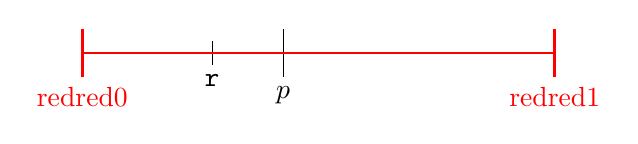
\begin{tikzpicture}[scale = 1.5, domain = -.5 : 6.5]
              \tikzstyle{mybox} = [rounded corners = 0pt] %
              \tikzstyle{fancytitle} = [rounded corners = 0pt] %
              \def\debSeg{0}; % la valeur de epsilon
              \def\finSeg{4}; % la valeur (exacte) de epsilon
              \def\color{red}; % la couleur choisie
              \def\r{1.1}; %
              \def\seuil{1.7};
              
              \draw[-] (\r,.1) -- (\r,-.1) node[below] {\tt r}; %
              \draw[-] (\seuil,.2) -- (\seuil,-.2) node[below] {$p$}; %

              \draw[-, very thick, color = \color] (\debSeg,.2) --
              (\debSeg,-.2) node[below] {$0$}; %
              \draw[-, very thick, color = \color] (\finSeg,.2) --
              (\finSeg,-.2) node[below] {$1$}; %
              
              \draw[-] (\debSeg, 0) -- (\finSeg, 0) ; % segment [0,1]
              
              \draw[-, color=\color, thick] ({\debSeg}, 0) -- ({\finSeg}, 0); %
            \end{tikzpicture}
          \end{center}
          On obtient une valeur plus petite que $p$ avec probabilité : 
          $\Prob(\Ev{ U \leq p}) = p$. \\
          On obtient une valeur strictement plus grande que $p$ avec
          probabilité :
          \[
          q = \Prob(\Ev{ U > p}) = 1 - \Prob(\Ev{ U \leq p}) = 1-p
          \]
          D'où le programme suivant :
          \begin{scilab}
            & \tcFun{function} \tcVar{res} = bernoulli(\tcVar{p})
            \nl %
            & \quad r = rand() \nl %
            & \quad \tcIf{if} r < \tcVar{p} \tcIf{then} \nl %
            & \quad \quad \tcVar{res} = 1 \nl %
            & \quad \tcIf{else} \nl %
            & \quad \quad \tcVar{res} = 0 \nl %
            & \quad \tcIf{end} \nl %
            & \tcFun{endfunction}
          \end{scilab}

      \item Plus généralement, cette méthode permet d'obtenir une
        simulation de n'importe quelle \var $X$ finie. Détaillons ce
        résultat. Soit $X$ une \var telle que :
        \begin{noliste}{$\stimes$}
        \item $X(\Omega) = \{ x_1, \ldots , x_n\}$,
        \item $\forall i \in \llb 1,n \rrb$, $\Prob(\Ev{X = x_i}) =
          p_i$.
        \end{noliste}
        L'idée est alors de découper le segment $[0, 1]$ en $n$
        intervalles $I_1$, \ldots, $I_n$.\\
        La taille du premier intervalle est $p_1$, celle du deuxième
        est $p_2$ et ainsi de suite.\\
        De sorte que, pour tout $i \in \llb 1, n \rrb$ :
        \[
        \Prob(\Ev{U \in I_i}) = p_i = \Prob(\Ev{X = x_i})
        \]
        Il n'y a plus qu'à écrire le programme correspondant.

      \item Afin de permettre une bonne compréhension des mécanismes
        en jeu, on a détaillé la réponse à cette question. Cependant,
        compléter correctement le programme \Scilab{} démontre la
        bonne compréhension de la simulation demandée et permet
        certainement d'obtenir tous les points alloués à cette
        question.\\
        On procédera de même dans les autres questions \Scilab{}.
        \end{noliste}        
      \end{remark}~\\[-1.4cm]
    \end{proof}


    \newpage


  \item Compléter la fonction suivante, qui effectue l'expérience
    étudiée avec une urne contenant initialement $b$ boules blanches,
    $n$ boules noires et qui ajoute éventuellement $c$ boules après le
    premier tirage,
    selon le choix de la variante dont le numéro est \texttt{variante}.\\
    Les paramètres de sortie sont~:
    \begin{noliste}{-}
    \item \texttt{x} : une simulation de la variable aléatoire $X$
    \item \texttt{y} : une simulation de la variable aléatoire $Y$
    \end{noliste}

    \begin{scilab}
      & \tcFun{function} [\tcVar{x}, \tcVar{y}] = experience (\tcVar{b}, 
      \tcVar{n}, \tcVar{c}, \tcVar{variante}) \nl %
      & \quad \tcVar{x} = tirage (\tcVar{b}, \tcVar{n}) \nl %
      & \quad \tcIf{if} \tcVar{variante} == 1 \tcIf{then} \nl %
      & \quad \quad \tcIf{if} \tcVar{x} == 1 \tcIf{then} \nl %
      & \quad \quad \quad ........... \nl %
      & \quad \quad \tcIf{else} \nl %
      & \quad \quad \quad ........... \nl %
      & \quad \quad \tcIf{end} \nl %
      & \quad \tcIf{else if} \tcVar{variante} == 2 \tcIf{then} \nl %
      & \quad \quad ........... \nl %
      & \quad \quad ........... \nl %
      & \quad \quad ........... \nl %
      & \quad \quad ........... \nl %
      & \quad \quad ........... \nl %
      & \quad \tcIf{end} \nl %
      & \quad \tcVar{y} = tirage (\tcVar{b}, \tcVar{n}) \nl %
      & \tcFun{endfunction}
    \end{scilab}
    
    \begin{proof}~
      \begin{noliste}{$\sbullet$}
      \item Comme on l'a vu dans la question précédente, l'instruction
        {\tt tirage(b, n)} permet de simuler la \var $X$. C'est ce que
        réalise l'instruction en ligne \ligne{2} du programme :
        \begin{scilabC}{1}
          & \quad \tcVar{x} = tirage (\tcVar{b}, \tcVar{n}) \nl %
        \end{scilabC}

      \item Il reste alors à simuler la \var $Y$.\\
        Le paramètre de sortie {\tt y} doit :
        \begin{noliste}{$\stimes$}
        \item prendre la valeur $1$ avec probabilité $\Prob(\Ev{Y =
            1}) = \dfrac{m}{m+d}$.
        \item prendre la valeur $2$ avec probabilité $\Prob(\Ev{Y =
            2}) = \dfrac{d}{m+d}$.
        \end{noliste}
        où $m$ (resp. $d$) représente le nombre de boules noires
        (resp. blanches) de l'urne après l'ajout éventuel issu du
        premier tirage.
      \item Plus précisément $m$ et $d$ sont définies en fonction du
        résultat du premier tirage et des variantes.\\
        {\bf Variante 1} : deux cas se présentent.
        \begin{noliste}{$\stimes$}
        \item \dashuline{Si {\tt x} vaut $1$} : c'est qu'on a tiré une
          boule noire lors du premier tirage.\\
          On remet, en plus de cette boule, $c$ boules noires dans
          l'urne. Ainsi : 
          \[
          m = n + c \quad \text{ et } \quad d = b \quad \text{(pas de
            modification)}
          \]
        \item \dashuline{Sinon ({\tt x} vaut $2$)} : c'est qu'on a
          tiré une boule blanche lors du premier tirage.\\
          On remet, en plus de cette boule, $c$ boules noires dans
          l'urne. Ainsi :
          \[
          m = n \quad \text{(pas de modification)} \quad \text{ et }
          \quad d = b + c
          \]          
        \end{noliste}


        \newpage


        \noindent
        On en déduit les lignes \ligne{3} à \ligne{8} du programme
        dans lesquelles on met à jour les variables {\tt n} et {\tt b}
        en fonction de leur nouvelle valeur.\\
        \begin{scilabC}{2}
          & \quad \tcIf{if} \tcVar{variante} == 1 \tcIf{then} \nl %
          & \quad \quad \tcIf{if} \tcVar{x} == 1 \tcIf{then} \nl %
          & \quad \quad \quad \tcVar{n} = \tcVar{n} + \tcVar{c} \nl %
          & \quad \quad \tcIf{else} \nl %
          & \quad \quad \quad \tcVar{b} = \tcVar{b} + \tcVar{c} \nl %
          & \quad \quad \tcIf{end} \nl %
        \end{scilabC}~\\
        {\bf Variante 2} : l'étude est similaire mais, comme on remet
        des boules de couleur opposée à la première boule tirée, les
        rôles de {\tt n} et {\tt b} sont échangés par rapport à la
        première variante. On en déduit les lignes \ligne{9} à
        \ligne{14} du programme dans lesquelles on met à jour les
        variables {\tt n} et {\tt b} en fonction de leur nouvelle
        valeur.\\
        \begin{scilabC}{8}
          & \quad \tcIf{else if} \tcVar{variante} == 2 \tcIf{then}
          \nl %
          & \quad \quad \tcIf{if} \tcVar{x} == 1 \tcIf{then} \nl %
          & \quad \quad \quad \tcVar{b} = \tcVar{b} + \tcVar{c} \nl %
          & \quad \quad \tcIf{else} \nl %
          & \quad \quad \quad \tcVar{n} = \tcVar{n} + \tcVar{c} \nl %
          & \quad \quad \tcIf{end} \nl %
        \end{scilabC}~\\
        {\bf Variante 3} : il n'y a pas de modifications des boules
        blanches ou noires. Il n'y a donc pas lieu de mettre à jour
        les variables {\tt n} et {\tt b}.
      \item On obtient alors la valeur {\tt y} en simulant le tirage
        dans l'urne modifiée (c'est à dire avec les valeurs de {\tt n}
        et {\tt b} mise à jour). C'est l'objectif de la ligne
        \ligne{16}.
        \begin{scilabC}{15}
          & \quad \tcVar{y} = tirage (\tcVar{b}, \tcVar{n}) \nl %
        \end{scilabC}
      \end{noliste}~\\[-1cm]
      % Détaillons le cas de la variante $1$.\\
      % La variable \texttt{n} correspond au nombre de boules noires
      % dans l'urne et \texttt{b} celui de boules blanches.
      % \begin{noliste}{$\sbullet$}
      % \item Si l'événement $\Ev{X=1}$ est réalisé, alors la boule
      %   piochée au $\er{1}$ tirage est noire.\\
      %   D'après l'énoncé, on ajoute donc \texttt{c} boules noires
      %   dans l'urne.  On met donc à jour le nombre de boules noires
      %   en lui ajoutant la valeur \texttt{c} : \texttt{n = n + c}
      % \item Si l'événement $\Ev{X=1}$ n'est pas réalisé, alors la
      %   boule
      %   piochée au $\er{1}$ tirage est blanche.\\
      %   D'après l'énoncé, on ajoute donc \texttt{c} boules blanches
      %   dans l'urne. On met donc à jour le nombre de boules blanches
      %   en lui ajoutant la valeur \texttt{c} : \texttt{b = b + c}
      % \end{noliste}
      % On procède de même pour la variante $2$.
      \begin{remark}
        \begin{noliste}{$\sbullet$}
        \item L'énoncé comporte une petite coquille. En effet, en
          ligne \ligne{9}, on devait lire :
          \begin{scilabC}{8}
            & \quad \tcIf{elseif} \tcVar{variante} == 2 \tcIf{then}
            \nl %
          \end{scilabC}
          en lieu et place de :
          \begin{scilabC}{8}
            & \quad \tcIf{else if} \tcVar{variante} == 2 \tcIf{then}
            \nl %
          \end{scilabC}
        \item La différence est subtile.
          \begin{noliste}{$-$}
          \item Dans le programme corrigé, la structure conditionnelle
            englobante contient $2$ branchements dont le $\eme{2}$ (en
            ligne \ligne{9}) est soumis à la condition {\tt
              \tcVar{variante} == 2}.
          \item Dans le programme d'origine, la structure
            conditionnelle englobante contient $2$ branchements dont
            le $\eme{2}$ (en ligne \ligne{9}) débouche sur une
            nouvelle structure conditionnelle {\tt \tcIf{if}
              \tcVar{variante} == 2}. Il faut alors fermer cette
            $\eme{2}$ structure conditionnelle à l'aide d'un {\tt
              \tcIf{end}}. Le nombre de lignes allouées n'est donc
            plus suffisant.
          \end{noliste}
        \item Notons que le respect du nombre de lignes alloué n'est
          pas déterminant. C'est plutôt une indication que donne le
          concepteur sur le nombre de lignes que le programme doit
          normalement prendre. Mais on peut raisonnablement penser que
          tout programme juste (même s'il ne respecte pas le nombre de
          lignes restant) sera accepté.
        \end{noliste}
      \end{remark}~\\[-1.4cm]
    \end{proof}


    \newpage


  \item Compléter la fonction suivante, qui simule l'expérience $N$
    fois (avec $N \in \N^*$), et qui estime la loi de $X$, la loi de
    $Y$ et la loi du couple $(X,Y)$.\\
    Les paramètres de sortie sont :
    \begin{noliste}{-}
    \item \texttt{loiX} : un tableau unidimensionnel à deux éléments qui 
      estime [ $\Prob(\Ev{X=1})$, \ $\Prob(\Ev{X=2})$ ]
    \item \texttt{loiY} : un tableau unidimensionnel à deux éléments qui 
      estime [ $\Prob(\Ev{Y=1})$, \ $\Prob(\Ev{Y=2})$ ]
    \item \texttt{loiXY} : un tableau bidimensionnel à deux lignes et
      deux colonnes qui estime :
      \[ 
      \left[ 
        \begin{array}{cc}
          \Prob(\Ev{X=1} \cap \Ev{Y=1}) &  \Prob(\Ev{X=1} \cap \Ev{Y=2})\\[.2cm]
          \Prob(\Ev{X=2} \cap \Ev{Y=2}) &  \Prob(\Ev{X=1} \cap \Ev{Y=2})  
        \end{array} 
      \right] 
      \]
    \end{noliste}
    \begin{scilab}
      & \tcFun{function} [\tcVar{loiX}, \tcVar{loiY}, \tcVar{loiXY}] =
      estimation(\tcVar{b}, \tcVar{n}, \tcVar{c}, \tcVar{variante},
      \tcVar{N}) \nl %
      & \quad \tcVar{loiX} = [0, 0] \nl %
      & \quad \tcVar{loiY} = [0, 0] \nl %
      & \quad \tcVar{loiXY} = [0, 0 ; 0, 0] \nl %
      & \quad \tcFor{for} k = 1 : \tcVar{N} \nl %
      & \quad \quad [x , y] = experience(\tcVar{b}, \tcVar{n}, \tcVar{c},
      \tcVar{variante}) \nl %
      & \quad \quad \tcVar{loiX}(x) = \tcVar{loiX}(x) + 1 \nl %
      & \quad \quad ........... \nl %
      & \quad \quad ........... \nl %
      & \quad \tcIf{end} \nl %
      & \quad \tcVar{loiX} = \tcVar{loiX} / \tcVar{N} \nl %
      & \quad \tcVar{loiY} = \tcVar{loiY} / \tcVar{N} \nl %
      & \quad \tcVar{loiXY} = \tcVar{loiXY} / \tcVar{N} \nl %
      & \tcFun{endfunction}
    \end{scilab}
    
    \begin{proof}~
      \begin{remark}%~\\
        L'énoncé de cette question comporte une erreur. \\
        Bien évidemment, la loi du couple $(X,Y)$ est caractérisé par la
        matrice :
        \[ 
        \left[ 
          \begin{array}{cc}
            \Prob(\Ev{X=1} \cap \Ev{Y=1}) &  \Prob(\Ev{X=1} \cap 
            \Ev{Y=2})\\[.2cm]
            \Prob(\Ev{X=2} \cap \Ev{Y=1}) &  \Prob(\Ev{X=2} \cap \Ev{Y=2})  
          \end{array} 
        \right] 
        \]
      \end{remark}
      \begin{noliste}{$\sbullet$}
      \item Dans la question précédente, on a simulé les \var $X$ et
        $Y$.\\
        Il s'agit maintenant d'obtenir une approximation des lois de
        ces \var

      \item Rappelons tout d'abord que $X$ ne prend que deux valeurs :
        $X(\Omega) = \{1, 2\}$.\\
        Ainsi, la loi de $X$ est entièrement déterminée par les
        valeurs :
        \[
        \Prob(\Ev{X = 1}) \quad \text{ et } \quad \Prob(\Ev{X = 2})
        \]
        L'idée naturelle pour obtenir un approximation de ces valeurs
        est : 
        \begin{noliste}{$\stimes$}
        \item de simuler un grand nombre de fois ($N$ est ce grand
          nombre) la \var $X$.\\
          Formellement, on souhaite obtenir un $N$-uplet $(x_1,
          \ldots, x_N)$ qui correspond à l'observation d'un
          $N$-échantillon $(X_1, \ldots, X_N)$ de la \var $X$.
        \item de compter le nombre de $1$ (resp. de $2$) de cette
          observation.          
        \end{noliste}
        Cette idée est justifiée par la loi faible des grands nombres
        (LfGN) qui affirme : 
        \[
        \dfrac{\text{nombre de $1$ de l'observation}}{\text{taille de
            l'observation}} \simeq \Prob(\Ev{X = 1})
        \]


        \newpage


      \item Dans le programme, les valeurs $(x_1, \ldots, x_N)$ sont
        obtenues par des appels successifs (à l'aide d'une boucle
        \texttt{for}) à la fonction {\tt experience} et stockées les
        unes après les autres dans la variable {\tt x}.
        \begin{scilabC}{4}
          & \quad \tcFor{for} k = 1 : \tcVar{N} \nl %
          & \quad \quad [x , y] = experience(\tcVar{b}, \tcVar{n},
          \tcVar{c}, \tcVar{variante}) \nl %
        \end{scilabC}
        {\it (seules les valeurs de {\tt x} nous intéressent dans un
          premier temps})\\
        Le tableau {\tt loiX} est alors mis à jour à chaque tour de
        boucle :
        \begin{scilabC}{6}
          & \quad \quad \tcVar{loiX}(x) = \tcVar{loiX}(x) + 1 \nl %
        \end{scilabC}
        Détaillons cette mise à jour : 
        \begin{noliste}{$\stimes$}
        \item \dashuline{si $\texttt{x}$ vaut $1$} alors
          l'instruction suivante est effectuée :
          \[
          \texttt{loiX(1) = loiX(1) + 1}
          \]
        \item \dashuline{si $\texttt{x}$ vaut $2$} alors l'instruction
          suivante est effectuée :
          \[
          \texttt{loiX(2) = loiX(2) + 1}
          \]
        \end{noliste}
        Cela signifie que le $\er{1}$ élément du tableau compte le
        nombre de $1$ de l'observation et que le $\eme{2}$ compte le
        nombre de $2$.\\        
        Une fois cette boucle effectuée, l'approximation formulée par
        la LfGN est obtenue en divisant ces nombres par la taille de
        l'observation :
        \begin{scilabC}{10}
          & \quad \tcVar{loiX} = \tcVar{loiX} / \tcVar{N} \nl %
        \end{scilabC}

      \item On agit de même pour obtenir l'approximation de la loi de
        $Y$.\\
        On génère des observations $(y_1, \ldots, y_N)$ d'un
        $N$-échantillon $(Y_1, \ldots, Y_N)$ de la \var $Y$.
        \begin{scilabC}{4}
          & \quad \tcFor{for} k = 1 : \tcVar{N} \nl %
          & \quad \quad [x , y] = experience(\tcVar{b}, \tcVar{n},
          \tcVar{c}, \tcVar{variante}) \nl %
        \end{scilabC}
        {\it (ce sont maintenant les valeurs de {\tt y} qui nous
          intéressent})\\ 
        Puis on met à jour le tableau {\tt loiY} de sorte à compter le
        nombre de $1$ et de $2$ que contient cette observation.
        \begin{scilabC}{7}
          & \quad \quad \tcVar{loiY}(y) = \tcVar{loiY}(y) + 1 \nl %
        \end{scilabC}
        L'approximation formulée par la LfGN est obtenue en divisant ces
        nombres par la taille de l'observation :
        \begin{scilabC}{11}
          & \quad \tcVar{loiY} = \tcVar{loiY} / \tcVar{N} \nl %
        \end{scilabC}

      \item On agit encore de même pour obtenir l'approximation de la
        loi de couple. On génère des couples d'observations $((x_1,
        y_1), \ldots, (x_N, y_N))$ d'un $N$-échantillon $((X_1, Y_1),
        \ldots, (X_N, Y_N))$ du couple $(X, Y)$. C'est toujours les
        lignes \ligne{5} et \ligne{6} :
        \begin{scilabC}{4}
          & \quad \tcFor{for} k = 1 : \tcVar{N} \nl %
          & \quad \quad [x , y] = experience(\tcVar{b}, \tcVar{n},
          \tcVar{c}, \tcVar{variante}) \nl %
        \end{scilabC}
        {\it (ce sont à présent les couples de valeurs qui nous
          intéressent)}\\ 
        Puis on met à jour le tableau {\tt loiXY} de sorte à compter
        le nombre de $(1,1)$, de $(1,2)$, de $(2,1)$, de $(2,2)$ :
        \begin{scilabC}{8}
          & \quad \quad \tcVar{loiXY}(x, y) = \tcVar{loiXY}(x, y) + 1 \nl %
        \end{scilabC}
        L'approximation formulée par la LfGN est obtenue en divisant ces
        nombres par la taille de l'observation :
        \begin{scilabC}{12}
          & \quad \tcVar{loiXY} = \tcVar{loiXY} / \tcVar{N} \nl %
        \end{scilabC}
      \end{noliste}~\\[-1cm]
    \end{proof}

  \item On exécute notre fonction précédente avec $b=1$, $n=2$, $c=1$,
    $N=10000$ et dans chacune des variantes. On obtient~:
    \[
    \begin{console}
      \lInv{[loiX,loiY,loiXY] = estimation(1,2,1,1,10000)} \nl %
      \lDisp{\qquad loiXY =} \nl %
      \lDisp{\qquad \qquad 0.49837 \qquad 0.16785} \nl %
      \lDisp{\qquad \qquad 0.16697 \qquad 0.16681} \nl %
      \lDisp{\qquad loiY =} \nl %
      \lDisp{\qquad \qquad 0.66534 \qquad 0.33466} \nl %
      \lDisp{\qquad loiX =} \nl %
      \lDisp{\qquad \qquad 0.66622 \qquad 0.33378} \nle %
      %%%%%
      \lInv{[loiX,loiY,loiXY] = estimation(1,2,1,2,10000)} \nl %
      \lDisp{\qquad loiXY =} \nl %
      \lDisp{\qquad \qquad 0.33258 \qquad 0.33286} \nl %
      \lDisp{\qquad \qquad 0.25031 \qquad 0.08425} \nl %
      \lDisp{\qquad loiY =} \nl %
      \lDisp{\qquad \qquad 0.58289 \qquad 0.41711} \nl %
      \lDisp{\qquad loiX =} \nl %
      \lDisp{\qquad \qquad 0.66544 \qquad 0.33456} \nle %
      %%%%%
      \lInv{[loiX,loiY,loiXY] = estimation(1,2,1,3,10000)} \nl %
      \lDisp{\qquad loiXY =} \nl %
      \lDisp{\qquad \qquad 0.44466 \qquad 0.22098} \nl %
      \lDisp{\qquad \qquad 0.22312 \qquad 0.11124} \nl %
      \lDisp{\qquad loiY =} \nl %
      \lDisp{\qquad \qquad 0.66778 \qquad 0.33222} \nl %
      \lDisp{\qquad loiX =} \nl %
      \lDisp{\qquad \qquad 0.66564 \qquad 0.33436} \nle %
    \end{console}
    \] 
    En étudiant ces résultats, émettre des conjectures quant à
    l'indépendance et l'échangeabilité de $X$ et $Y$ dans chacune des
    variantes. \\
    On donne les valeurs numériques approchées suivantes~:
    \[ 
    \begin{array}{l}
      0.33 \times 0.33 \simeq 0.11 \\
      0.33 \times 0.41 \simeq 0.14 \\
      0.33 \times 0.58 \simeq 0.19 \\
      0.33 \times 0.66 \simeq 0.22 \\
      0.41 \times 0.66 \simeq 0.27 \\
      0.58 \times 0.66 \simeq 0.38 \\
      0.66 \times 0.66 \simeq 0.44 
    \end{array} 
    \]
    
\begin{proof}~ 
  \begin{noliste}{$\sbullet$}
    \item {\bf Variante 1} :
    \begin{noliste}{$\stimes$}
    \item \dashuline{Indépendance}.
    On lit $\Prob(\Ev{X=1} \cap \Ev{Y=1})$ sur la coordonnée $(1,1)$ 
    de \texttt{loiXY}. \\[.2cm]
    Donc : $\Prob(\Ev{X=1} \cap \Ev{Y=1}) \simeq 
    0,49$\\[.2cm]
    On lit $\Prob(\Ev{X=1})$ sur la $\ere{1}$ coordonnée de 
    \texttt{loiX}. Donc $\Prob(\Ev{X=1}) \simeq 0,66$.
    

    \newpage

    
    On lit $\Prob(\Ev{Y=1})$ sur la $\ere{1}$ coordonnée de 
    \texttt{loiX}. Donc $\Prob(\Ev{Y=1}) \simeq 0,66$.\\[.2cm]
    D'après les données de l'énoncé, on obtient donc :
    \[
     \Prob(\Ev{X=1}) \Prob(\Ev{Y=1}) \simeq 0,44 \neq 
     \Prob(\Ev{X=1} \cap \Ev{Y=1})
    \]
    On conjecture alors que $X$ et $Y$ ne sont pas indépendantes.
    
    \item \dashuline{Échangeabilité}.
    On lit $\Prob(\Ev{X=1} \cap \Ev{Y=2})$ sur la coordonnée $(1,2)$ 
    de \texttt{loiXY}, et \\[.2cm]
    $\Prob(\Ev{X=2} \cap \Ev{Y=1})$ sur la 
    coordonnée $(2,1)$ de \texttt{loiXY}. Donc :
    \[
     \Prob(\Ev{X=1} \cap \Ev{Y=2}) \simeq 
    0,16 \simeq \Prob(\Ev{X=1} \cap \Ev{Y=2})
    \]
    On conjecture alors que $X$ et $Y$ sont échangeables.
    \end{noliste}
    \conc{Dans le cas de la variante 1, on conjecture que les \var $X$ 
    et $Y$ sont \\
    échangeables et non indépendantes.}
    
    \item {\bf Variante 2} :
    \begin{noliste}{$\stimes$}
    \item \dashuline{Indépendance}. Par lecture : $\Prob(\Ev{X=1} \cap 
    \Ev{Y=1}) \simeq 0,33$\\[.2cm]
    De plus : $\Prob(\Ev{X=1}) \simeq 0,66$ et $\Prob(\Ev{Y=1}) \simeq 
    0,58$.\\[.2cm]
    D'après les données de l'énoncé, on obtient donc :
    \[
     \Prob(\Ev{X=1}) \Prob(\Ev{Y=1}) \simeq 0,38 \neq 
     \Prob(\Ev{X=1} \cap \Ev{Y=1})
    \]
    On conjecture alors que $X$ et $Y$ ne sont pas indépendantes.
    
    \item \dashuline{Échangeabilité}. Par lecture :
    $\Prob(\Ev{X=1}\cap \Ev{Y=2}) \simeq 0,33$ et
    $\Prob(\Ev{X=2} \cap \Ev{Y=1}) \simeq 0,25$.\\[.2cm]
    Donc : $\Prob(\Ev{X=1}\cap \Ev{Y=2}) \neq 
    \Prob(\Ev{X=2}\cap \Ev{Y=1})$.\\[.2cm]
    On conjecture alors que $X$ et $Y$ ne sont pas échangeables.
    \end{noliste}
    \conc{Dans le cas de la variante 2, on conjecture que les \var $X$ 
    et $Y$ sont \\
    non échangeables et non indépendantes.}
    
    \item {\bf Variante 3} : 
    \begin{noliste}{$\stimes$}
    \item \dashuline{Indépendance}. Par lecture :
    \[
     \Prob(\Ev{X=1}) \Prob(\Ev{Y=1}) \simeq 0,66 \times 0,66
     \simeq 0,44 \simeq \Prob(\Ev{X=1} \cap \Ev{Y=1})
    \]
    \[
     \Prob(\Ev{X=1}) \Prob(\Ev{Y=2}) \simeq 0,66 \times 0,33
     \simeq 0,22 \simeq \Prob(\Ev{X=1} \cap \Ev{Y=2})
    \]
    \[
     \Prob(\Ev{X=2}) \Prob(\Ev{Y=1}) \simeq 0,33 \times 0,66
     \simeq 0,22 \simeq \Prob(\Ev{X=2} \cap \Ev{Y=1})
    \]
    \[
     \Prob(\Ev{X=2}) \Prob(\Ev{Y=2}) \simeq 0,33 \times 0,33
     \simeq 0,11 \simeq \Prob(\Ev{X=2} \cap \Ev{Y=2})
    \]
    On conjecture alors que $X$ et $Y$ sont indépendantes.
    
    \item \dashuline{Échangeabilité}. Par lecture :
    \[
     \Prob(\Ev{X=1} \cap \Ev{Y=2}) \simeq 
     0,22 \simeq \Prob(\Ev{X=1} \cap \Ev{Y=2})
    \]
    On conjecture alors que $X$ et $Y$ sont échangeables.
    \end{noliste}
    \conc{Dans le cas de la variante 3, on conjecture que les \var $X$ 
    et $Y$ sont \\
    échangeables et indépendantes.}
  \end{noliste}
\end{proof}



\newpage



\end{noliste}
\item On se place dans cette question dans le cadre de la variante $1$.
\begin{noliste}{a)}
\item Donner la loi de $X$.


\begin{proof}~
 \begin{noliste}{$\sbullet$}
  \item Par définition de la \var $X$ : $X(\Omega)=\{1,2\}$.
  
  \item L'événement $\Ev{X=1}$ est réalisé par tous les tirages d'une
    boule de l'urne dont le résultat est une boule noire.\\
    Un tel $1$-tirage est entièrement déterminé par la boule noire choisie.\\
    Il y a donc $n$ tels $1$-tirages possibles (autant que de boules
    noires).\\
    De plus, le nombre total de $1$-tirages possibles est $n+b$
    (autant que de boules dans l'urne).\\[.2cm]
    On obtient alors : $\Prob(\Ev{X=1})=\dfrac{n}{n+b}$.
  
  \item La famille $(\Ev{X=1}, \Ev{X=2})$ est un système complet 
  d'événements. Donc :
  \[
   \Prob(\Ev{X=2})=1-\Prob(\Ev{X=1}) = 1-\dfrac{n}{n+b} =
   \dfrac{b}{n+b}
  \]
 \end{noliste}
 \conc{Ainsi, $X(\Omega)=\{1,2\}$. De plus :
   $\Prob(\Ev{X=1})=\dfrac{n}{n+b}$ \ et \
   $\Prob(\Ev{X=2})=\dfrac{b}{n+b}$.}~\\[-1cm]
\end{proof}



\item Déterminer la loi du couple $(X,Y)$.

\begin{proof}~
  \begin{noliste}{$\sbullet$}
  \item On sait déjà : $X(\Omega)=\{1,2\}$. Par définition de la \var
    $Y$, on a aussi : $Y(\Omega)=\{1,2\}$.
  
  \item Déterminons tout d'abord $\Prob_{\Ev{X=1}}(\Ev{Y = 1})$.\\[.2cm]
    Si l'événement $\Ev{X=1}$ est réalisé, c'est que la $\ere{1}$
    boule tirée est noire. On se place dans le cadre de la variante
    $1$ donc, à l'issue de ce tirage, $c$ boules noires sont ajoutées
    dans l'urne.\\
    L'événement $\Ev{Y=1}$ est alors réalisé par tous les tirages
    d'une boule de l'urne dont le résultat est une boule noire.\\
    Un tel $1$-tirage est entièrement déterminé par la boule noire
    choisie.\\
    Il y a donc $n + c$ tels $1$-tirages possibles (autant que de
    boules noires).\\
    De plus, le nombre total de $1$-tirages possibles est maintenant
    de $n+b+c$ (autant que de boules dans l'urne). %
    \conc{On en conclut :
      $\Prob_{\Ev{X=1}}(\Ev{Y=1})=\dfrac{n+c}{n+b+c}$}%
    (on remarque que la probabilité conditionnelle est bien définie
    car $\Prob(\Ev{X=1})=\dfrac{n}{n+b} \neq 0$)
    
  \item Déterminons alors $\Prob_{\Ev{X=1}}(\Ev{Y = 2})$.\\
    La famille $(\Ev{Y=1}, \Ev{Y=2})$ est un système complet
    d'événements. Donc :
    \[
    \Prob_{\Ev{X=1}}(\Ev{Y=2}) = 1- \Prob_{\Ev{X=1}}(\Ev{Y=1}) = 1-
    \dfrac{n+c}{n+b+c} = \dfrac{b}{n+b+c}
    \]
    \conc{$\Prob_{\Ev{X=1}}(\Ev{Y=2}) = \dfrac{b}{n+b+c}$}

  \item Avec les mêmes raisonnements, on obtient : %
    \conc{ $\Prob_{\Ev{X=2}}(\Ev{Y=1})=\dfrac{n}{n+b+c} \quad \mbox{
        et } \quad \Prob_{\Ev{X=2}}(\Ev{Y=2})=\dfrac{b+c}{n+b+c}$}%
    (les probabilités conditionnelles sont bien définies car
    $\Prob(\Ev{X=2})=\dfrac{b}{n+b} \neq 0$)
        
  \item On a alors les résultats suivants :
  \[
   \Prob(\Ev{X=1}\cap \Ev{Y=1}) = \Prob(\Ev{X=1}) \times 
   \Prob_{\Ev{X=1}}(\Ev{Y=1}) = \dfrac{n}{n+b} \times 
   \dfrac{n+c}{n+b+c} = \dfrac{n(n+c)}{(n+b)(n+b+c)}
  \]
  
  \[
   \Prob(\Ev{X=1}\cap \Ev{Y=2}) = \Prob(\Ev{X=1}) \times 
   \Prob_{\Ev{X=1}}(\Ev{Y=2}) = \dfrac{n}{n+b} \times 
   \dfrac{b}{n+b+c} = \dfrac{n \, b}{(n+b)(n+b+c)}
  \]
  
  \[
   \Prob(\Ev{X=2}\cap \Ev{Y=1}) = \Prob(\Ev{X=2}) \times 
   \Prob_{\Ev{X=2}}(\Ev{Y=1}) = \dfrac{b}{n+b} \times 
   \dfrac{n}{n+b+c} = \dfrac{n \, b}{(n+b)(n+b+c)}
  \]
  
  \[
   \Prob(\Ev{X=2}\cap \Ev{Y=2}) = \Prob(\Ev{X=2}) \times 
   \Prob_{\Ev{X=2}}(\Ev{Y=2}) = \dfrac{b}{n+b} \times 
   \dfrac{b+c}{n+b+c} = \dfrac{b(b+c)}{(n+b)(n+b+c)}
  \]
  
  
  \item En résumé, la loi du couple $(X, Y)$ est donnée par le
        tableau suivant.\\[.4cm]
        \[
        % \renewcommand{\arraystretch}{1.5}
        \begin{tabular}{|>{\centering\arraybackslash\small}c||
            *{2}{>{\centering\arraybackslash\small$}m{3cm}<{$}|}}
          % \hhline{~|*{3}{-}}
          \hline
          \diagbox[width=2cm, height=1.6cm]
          {\scalebox{.8}{$x \in X(\Omega)$}}
          {\hspace*{-.2cm}\scalebox{.8}{$y \in Y(\Omega)$}}
          & \cellcolor{gray!20} 1 & \cellcolor{gray!20} 2
          \\
          \hline
          \hline
          \rule[18pt]{0pt}{0pt}
          \cellcolor{gray!20} 1
          \rule[-15pt]{0pt}{0pt} 
          & \dfrac{n(n+c)}{(n+b)(n+b+c)} & \dfrac{n \, b}{(n+b)(n+b+c)}
          \\
          \hline
          \rule[18pt]{0pt}{0pt}
          \cellcolor{gray!20} 2
          \rule[-15pt]{0pt}{0pt} 
          & \dfrac{n \, b}{(n+b)(n+b+c)} & \dfrac{b(b+c)}{(n+b)(n+b+c)} 
	  \\
        \hline
      \end{tabular}
      \]~\\[-.6cm]      
 \end{noliste}
 
 \begin{remark}
  On peut remarquer dès cette question que les \var $X$ et $Y$ sont 
  échangeables.
 \end{remark}~\\[-1.4cm]
\end{proof}


\item Déterminer la loi de $Y$.

\begin{proof}~
 \begin{noliste}{$\sbullet$}
  \item On rappelle : $Y(\Omega)=\{1,2\}$.
  
  \item La famille $(\Ev{X=1},\Ev{X=2})$ forme un système complet
    d'événements.\\
    On en déduit, par application de la formule des probabilités
    totales :
    \[
    \begin{array}{rcl}
      \Prob(\Ev{Y=1}) & = & \Prob(\Ev{X=1} \cap \Ev{Y=1}) + 
      \Prob(\Ev{X=2}\cap \Ev{Y=1})
      \\[.2cm]
      & = & \dfrac{n(n+c)}{(n+b)(n+b+c)} + \dfrac{n \, b}{(n+b)(n+b+c)}
      \\[.6cm]
      & = & \dfrac{n\, \bcancel{(n+c+b)}}{(n+b)\bcancel{(n+b+c)}}
      \ = \ \dfrac{n}{n+b}
    \end{array}
    \]
  
  \item La famille $(\Ev{Y=1},\Ev{Y=2})$ forme un système complet 
  d'événements. Donc :
  \[
   \Prob(\Ev{Y=2}) = 1-\Prob(\Ev{Y=1}) = 1-\dfrac{n}{n+b} = 
   \dfrac{b}{n+b}
  \]
 \end{noliste}
 \conc{Ainsi, $Y(\Omega)=\{1,2\}$. De plus :
   $\Prob(\Ev{Y=1})=\dfrac{n}{n+b}$ \ et \
   $\Prob(\Ev{Y=2})=\dfrac{b}{n+b}$.}
 
 
 \newpage
 
 
 
 \begin{remark}
  \begin{noliste}{$\sbullet$}
  \item On constate que $Y$ suit la même loi que $X$.\\
    Ceci est tout à fait normal puisqu'on a remarqué à la question
    précédente que $X$ et $Y$ sont échangeables. Or, d'après la
    question \itbf{2.}, si $X$ et $Y$ sont échangeables, alors $X$ et
    $Y$ ont même loi.
  \item Cependant, l'énoncé attendait vraiment ici l'utilisation de la
    formule des probabilités totales pour déterminer la loi de la \var
    $Y$. En effet, le caractère échangeable de $X$ et $Y$ est demandé
    à la question suivante.
  \end{noliste}
\end{remark}~\\[-1.4cm]
\end{proof}


\item Montrer que $X$ et $Y$ sont échangeables mais ne sont pas 
indépendantes.

\begin{proof}~
 \begin{noliste}{$\sbullet$}
  \item \dashuline{Échangeabilité}.
  \[
   \Prob(\Ev{X=1}\cap \Ev{Y=2}) = \dfrac{n \, b}{(n+b)(n+b+c)} =
   \Prob(\Ev{X=2}\cap \Ev{Y=1})
  \]
  \conc{On en déduit que $X$ et $Y$ sont échangeables.}
  
  \item \dashuline{Indépendance}.
  \[
   \Prob(\Ev{X=1}) \times \Prob(\Ev{Y=2}) = \dfrac{n}{n+b} \times 
   \dfrac{b}{n+b} = \dfrac{n\, b}{(n+b)^2}
  \]
  De plus : $\Prob(\Ev{X=1}\cap \Ev{Y=2}) = \dfrac{n\, 
  b}{(n+b)(n+b+c)}$\\[.2cm]
  On a alors les équivalences suivantes :
  \[
   \begin{array}{rcl}
    & & \Prob(\Ev{X=1}\cap \Ev{Y=2}) = \Prob(\Ev{X=1}) \times 
    \Prob(\Ev{Y=2})
    \\[.2cm]
    & \Leftrightarrow & \dfrac{n\, b}{(n+b)(n+b+c)} = \dfrac{n\, b}
    {(n+b)^2}
    \\[.6cm]
    & \Leftrightarrow & n+b = n+b+c
    \\[.2cm]
    & \Leftrightarrow & c=0
   \end{array}
  \]
  Or, d'après l'énoncé : $c\neq 0$ (on a même : $c>0$). Ainsi :
  \[
   \Prob(\Ev{X=1}\cap \Ev{Y=2}) \neq \Prob(\Ev{X=1}) \times 
   \Prob(\Ev{Y=2})
  \]
  \conc{On en déduit que $X$ et $Y$ ne sont pas indépendantes.}~\\[-.9cm]
 \end{noliste}
 \begin{remark}
  Récapitulons ce que l'on a démontré dans cet exercice.
  \begin{noliste}{$\sbullet$}
    \item En question \itbf{1.}, on a montré l'implication :
      \[
      \mbox{$X$ et $Y$ sont indépendantes et de même loi \
        $\Rightarrow$ \ $X$ et $Y$ sont échangeables}
      \]
    
    \item En question \itbf{2.}, on a montré l'implication :
      \[
      \mbox{$X$ et $Y$ sont échangeables \ $\Rightarrow$ \ $X$ et $Y$
        ont même loi}
      \]
    
    \item Les questions \itbf{3.} et \itbf{4.} consistaient à
      démontrer (en exhibant un contre-exemple) :
      \[
      \mbox{$X$ et $Y$ sont échangeables \quad
        \bcancel{\rule[-.2cm]{0cm}{.2cm} \!\!\! $\Rightarrow$ \!\!\!
          \rule[-.2cm]{0cm}{.2cm}} \quad $X$ et $Y$ sont
        indépendantes}
      \]      
  \end{noliste}
 \end{remark}~\\[-1.4cm]
\end{proof}

\end{noliste}
\end{noliste}

